% =====================================================================
%  MIG 2026 SHORT PAPER  (4-6 pages EXCLUDING references, per the CFP)
%
%  Builds with:  latexmk -pdf onesweep_short.tex
%
%  This is a NEW, self-contained short paper. It shares only the acmart
%  preamble skeleton with main_short.tex; it does not fork its sections and
%  does not restate its claims. main_short.tex is the companion diagnosis
%  paper and is never modified from here.
%
%  NUMBER PROVENANCE. Every headline number traces to a CSV under
%  benchmarks/paper_eval/t_onesweep/out/ (the T-suite, git_sha e58083a):
%   - boundary (omega h)^2 = 1 + m/M, 0 of 58081 cells misclassified, the
%     boundary reproduced exactly          <- t2_phasemap.csv
%   - identity battery rel <= 1e-12, 29/29 checks; E+/E- = 25.5 note vector;
%     implicit Delta E = -0.4950980 note vector   <- t1_identities.csv
%   - nonmodal collapse 288/288 sign, max|y-(rho-1)| = 4.26e-14, 4 variants,
%     no modal basis anywhere              <- t3_nonmodal.csv
%   - ordering divisor (1+b)^2 = 10201 at b=100 exact, D_B/D_A exact,
%     converged endpoint passive           <- t5_ordering.csv
%   - reconstruction-general ordering (T5 carried through kappa): D_B/D_A =
%     (1+b)^2 at EVERY kappa; trailing spring injects iff (kappa^2+b)/(1+b)^2 >
%     2 + m/M, hence passive for all b at kappa=1 (0 of 10,000 cells) and
%     injecting on 3840 of 10,000 at kappa=2 over b in [1e-3,1e2] x m/M in
%     [1e-2,10]; band b < b* = 2(kappa^2-s)/(sqrt(1+4s(kappa^2-1))+2s-1),
%     s = 2+m/M, nonempty iff m < (kappa^2-2)M; b* = (sqrt(37)-5)/6 = 0.18046 at
%     m=M, which at the shipped h = 1/960 s is every mode below 64.91 Hz; peak
%     deposit (kappa^2-2)^2/(4(kappa^2-1)) = exactly 1/3 of E- at kappa=2,
%     m=M/2, b->0. The kappa=1 slice reproduces run_t5_ordering.py and
%     t5_ordering.csv BIT-IDENTICALLY (max abs diff 0.0). Tolerances: 8.0e-16
%     scale-normalized on all 40,000 cells, 1.9e-13 pure-relative on the 39,956
%     with injection margin >= 1e-3, and 600 exact-rational cells at ZERO
%     tolerance including cells 1e-9 either side of b*
%                                          <- t13_ordering_kappa.csv
%   - shipped row: BE control 27/27 mass sign + 27/27 implicit passive;
%     symplectic reconstruction factor 2.000 (4x modal KE); midpoint index
%     27/27; implicit under midpoint dinner 9/9, shelf 2/9, ledge 4/9
%                                          <- t4_shipped.csv
%   - system corroboration on the MODAL-OVERRUN metric (a cell overruns when
%     peak modal energy / peak impactor rigid KE > 1; this is NOT the E+ > E-
%     sign of Sec. 2, and the body now says so): 8/24 explicit overrun ->
%     0/24 implicit; worst ratios ledge 1.2e5, shelf 1.1e4
%                                          <- weight_swap_full.csv
%                                            (summarized t6_ews_corroboration.csv)
%     A direct per-substep TOTAL mechanical-energy readout of the same 24-cell
%     grid, PRINTED in Sec. 4 as "the total-energy sign gives 10, 1 and 0 of 24
%     across the three arms": cells with a net energy excess above the window
%     start (i.e. the theorem's own E+ > E- sign, not the modal ratio) are 10/24
%     explicit, 1/24 backward-Euler (that one at 1.2e-5 of the impactor KE) and
%     0/24 matched; the position-based update's ballistic drift makes those
%     counts lower bounds
%                                          <- x1_passivity/out/weight_swap_energy.csv
%                                             (run_weight_swap_energy.py)
%   - reconstruction-general effective mass mu = m(kappa^2 + (omega h)^2), the
%     dE formula and the matched-weight inelastic identity, 7000 cells at
%     rel <= 1e-12, 0 sign mismatches; kappa=1 -> m(1+b), kappa=2 -> m(4+b)
%                                          <- t7_reconstruction.csv
%   - shipped-convention relaxation boundary theta^2(kappa^2 + b) = 2 + m/M,
%     deposit scales theta^2, 542 injecting->passive, 0 passive->injecting
%                                          <- t8_relaxation.csv
%   - shipped row, symplectic default, reconstruction-matched weight
%     m(4 + (omega h)^2) = 4 M_q + h^2 K_q: 27/27 passive, matched index < 1
%                                          <- t4_matched.csv
%   - rho_mid = (L + 2 sum a_i)/(w_r + 2 a_tilde) tracks 27/27 while the
%     backward-Euler rho tracks 22/27 with 5 FALSE NEGATIVES (the unsafe
%     direction)                           <- t4_index_audit.csv
%   - multi-coordinate operator form: matched charge (kappa^2 M_c + h^2 K_c)^-1
%     passive 3000/3000 float cells and EXACT on 300/300 rational cells;
%     diagonal-only charge on non-diagonal K_c injects 19/2000
%                                          <- t10_multimode.csv
%   - T10 attempted-cell count 9900 float = A 1500 + B 3000 + C 800*3 + D 2000
%     + D 1000, plus 300 exact-rational cells (the governing exactness check);
%     the shipped CSV records the 5000 per-cell rows of blocks B and D
%                                          <- t10_multimode.csv
%   - accuracy vs the converged reference: C+ = 0 for every weight (2.1e-16 of
%     |hv|); matched sweep == converged backward-Euler step to 5.5e-16 on
%     impulse, v+, q+, qdot+; damped gap 0.979 zeta omega h; mass-only
%     over-deposit (M+m(1+b))/(M+m) = 5001 at b = 1e4; matched kappa=2 charge
%     m(4+b) == 4 m(1+b/4), never less dissipative than the reference on
%     3000/3000 cells                      <- t11_accuracy.csv
%   - three-arm system weight swap on the production host (same overrun metric
%     as above): explicit 8/24 overrunning (worst 1.195e5, ledge 4x1 relax 1.0),
%     backward-Euler 0/24, MATCHED (4M_q+h^2K_q) 0/24 (worst ratio 0.109) and
%     strictly
%     below the backward-Euler arm on all 24; explicit arm reproduces the
%     companion CSV to 0.0 relative
%                                          <- weight_swap_matched.csv
%   - hypothesis pinning (new T12 arm, run_t12_hypotheses.py, from-scratch sweep
%     sharing no code with the other T scripts): the reconstruction-split form
%     dE = (v^2/2D^2)[u'Gu - kappa_r(2-kappa_r) w_r - 2 kappa_r (J_c'u + alpha~)]
%     at rel 5.5e-14 on 9000 cells (n = 1..4, dense K_c, kappa and kappa_r in
%     [0.1,4], alpha~ mixed, three charges), kappa_r = 1 recovering the printed
%     dE term for term; mass-only boundary kappa^2 + b = 2 kappa_r +
%     kappa_r(2-kappa_r) m/M with 0 of 4000 misclassified at each of
%     (kappa_r,kappa) = (1,1), (1,2), (2,2), (2,1), (3,3); matched charge passive
%     for every kappa at kappa_r = 1 (6000 cells, |kappa| in [1e-3,1e3], worst
%     dE/E- = -7.6e-10) and, under kappa_r = kappa, passive at every mass ratio
%     iff kappa in [1/2,2] (0 of 2000 injecting at 0.5, 0.75, 1, 2; 1268 of 2000
%     at 0.4; 1039 of 2000 at 3; endpoints 0.4999 and 2.0001 both inject);
%     over-deposit 1 + b m/(M+m) tabulated over m/M, so 1.5 / 51 / 5001 is the
%     m = M row (m/M = 0.01 gives 1.010 / 1.990 / 100.01); damped amplitude gap
%     exactly 2 zeta omega h/(1 + M/m + b), rel 5.1e-16 on 4000 cells, equal to
%     0.979 zeta omega h at the T11 point M = m = 1, omega = 50, h = 1/240
%     (b = 0.043); the kappa = 2 converged reference reproduced by the row charge
%     mu* = 2 m(1 + b/4) = m(2 + b/2) on impulse, v+, q+ and qdot+ at 4.3e-16,
%     the matched m(4+b) being exactly 2 mu* (0.0 relative) with amplitude ratio
%     (M+mu*)/(M+2mu*) measured inside (0.5, 1); kappa = 1 exactness verified for
%     n = 1..4 with dense K_c at 4.4e-16 and requiring zeta = 0
%                                          <- t12_hypotheses.csv
%   - the 24-cell grid's budgets are ITERATIONS x SUBSTEPS per 1/120 s FRAME, so
%     the substep h of Sec. 2 is 1/120, 1/240, 1/480, 1/960 s at (4,1), (8,2),
%     (16,4), (32,8); the body states that range rather than "at h = 1/120"
%                                          <- weight_swap_full.csv, h_sub column
%   - the shipped host recovers rigid velocity as (x - x_prev)/h (kappa_r = 1)
%     for every body and commits the mode at the midpoint 2(q - q^n)/h - qdot^n
%     (kappa = 2), so every shipped-row result is the mixed (1, 2) case
%                                          <- solver velocity-update block
%                                             (shipped in the supplement)
%   - TEASER (Fig. 1), read from the frozen shelf-scene recording
%     out/onesweep_scene_data/onesweep_scene_traj.npz + scene_data_summary.json
%     (onesweep_scene_record.py, git_sha e58083a; NOT a T-suite CSV): board-mode
%     energy at the displayed substep 541, unfixed 1707.1965 J -> "1,707 J" and
%     matched 0.3546 J -> "0.35 J"; peak book rise unfixed 56.82268 mm ->
%     "56.8 mm", matched 5.27887 mm -> "5.3 mm", converged 32x8 reference arm
%     9.64714 mm -> "9.6 mm"; scene 6.0 kg dropped 1.0 m onto FIVE standing
%     books (scene reduced_shelf, n_bodies 6, book_rise_per_book_mm has 5
%     entries, of which 56.82268 is the max); operating point
%     1 iteration x 8 substeps at h_frame = 1/120 s, governor off, kappa = 2.
%     The teaser row's own danger index at its own operating point (steel board,
%     200 GPa / 7850 kg m^-3, h = 1/960 s) is rho = 7.1e3..7.5e3 and
%     rho_mid = 8.6e3..9.0e3 over its eight impactor support rows, all > 1. NOT
%     the T4 shelf s=1 figure (rho = 6.65e4), which is a soft 0.5 GPa board at
%     h = 1/120 s.                         <- scene_params_cells.csv
%   - TABLE 1 CELL/RESULT COLUMNS. T1 29 checks over 2626 case-instances (26
%     binding, 3 report-only), all pass    <- t1_identities.csv
%     T3 300 cells = 4 variants x 3 mass ratios x 25 stiffness targets; 12 are
%     the exact rho = 1 cells of the logspace grid and are non-live, each with
%     |dE| <= 1.11e-16 = 2.22e-16 of E- = 0.5 J
%                                          <- t3_nonmodal.csv
%     T4 63 rows = 27 mass + 27 implicit at iterations 1, plus a 9-cell
%     shelf-only iteration annex; all 63 isolation-valid
%                                          <- t4_shipped.csv
%     T5 208 runs = 8 (M,m,b) cells x 2 orders x (12 sweep counts + 1
%     converged); 184/184 checks pass      <- t5_ordering.csv
%     T7 7000 = block (a); the row's 21 checks span 42767 case-instances
%                                          <- t7_reconstruction.csv
%     T8 1200 = shipped-convention block (inject 323 / passive 877, 0 sign
%     mismatches); 1600 = direction block (0 passive->injecting, 542 safe
%     injecting->passive); 14 checks over 14523 case-instances
%                                          <- t8_relaxation.csv
%     T10 17/17 checks; 9900 float cells (A 1500 + B 3000 + C 800*3 + D 2000
%     + D 1000) at atol 1e-9, a further 12000-cell block-F conditioning
%     staircase, and 300 exact-rational cells (block E, 0 skipped)
%                                          <- t10_multimode.csv
%     T11 8/8 checks over 15000 draws (4000 + 4000 + 2000 + 2000 + 3000); the
%     first block expands 4000 draws x 2 kappa x 4 weights = the 32000
%     arm-cells quoted in the text; the CSV ships only the 16 deterministic
%     tabulated cells                      <- t11_accuracy.csv
%     T13 40,000 cells = 2 kappa x 2 orders x 100 b x 100 m/M; the tabulated
%     0 and 3840 are the trailing-spring (order A) arm, 10,000 cells each
%                                          <- t13_ordering_kappa.csv
%
%  ---- ADDED 2026-07-28 (evidence-integration pass). Three new T14 arms. ----
%
%   - PASSIVE FAMILY (Cor. 3.4, run_t14_passive_family.py). W = c G^-1 with
%     G = kappa^2 M_c + h^2 K_c; substituting into Eq. (6) telescopes BOTH
%     bracket terms through a = J_c' G^-1 J_c, giving
%     dE = (v^2/2D^2)[c(c-2) a - w_r - 2 a_tilde], D = w_r + c a + a_tilde,
%     so c(c-2) <= 0 on exactly [0,2]. Operator form: u'Gu <= 2 J_c'u for every
%     row direction reads W G W <= 2W, equivalent for symmetric W and G > 0 to
%     the Loewner interval 0 <= W <= 2 G^-1.
%     * [CUT FROM THE BODY 2026-07-28 in the length pass; RESTORABLE verbatim if
%       space ever appears] "no cell of 1500 scalar and 600 multi-mode injects
%       anywhere in [0,2] at any of 22 values of c" = blocks A_scalar and
%       B_multimode, n_inject = 0
%       for every c in {0, 1e-9, .25, .5, .75, 1, 1.25, 1.5, 1.75, 1.9, 1.99,
%       1.999999999, 2}; outside, 254/1500 and 145/600 inject at c = 2.01,
%       805/1500 at c = -1 and 917/1500 at c = 4. n_pred_inject == n_inject on
%       every row, so the closed form calls the measured sign exactly. The ray
%       measurement was cut rather than the operator one because
%       C_operator_interval (below) is the stronger of the two: it tests the
%       Loewner iff in both directions, the ray only along W = c G^-1
%   - * "2500 randomized symmetric charges each met with an adversarial row
%       direction, all 1222 inside the interval passive and all 1278 outside
%       injecting" = block C_operator_interval. The 1278 is the SHARPNESS of
%       the iff: for every W outside the interval a row direction that injects
%       is constructed and then measured
%     * [CUT FROM THE BODY 2026-07-28 in the length pass, D2's drop item (1);
%       RESTORABLE] "halving the diagonal charge restores passivity on all 2000
%       of those rows" = block G3_diag_on_coupled, the diagonal-only charge on coupled
%       K_c: inject 16/2000 at c = 1, 2/2000 at c = 0.75, 0/2000 at c = 0.5 and
%       c = 0.25. (The body's separate "19 of 2000" is tcost_charges.csv, a
%       DIFFERENT 2000-cell draw; the two counts are not the same experiment
%       and must not be merged.) The safe band is c = 2B/A with A = d'Gd,
%       B = J_c'd, d = diag(G)^-1 J_c: median 2.002, 5th pct 1.120, below 1 on
%       3.05% of cells (block G3_band)
%     * "the far endpoint c = 2 is G/2, which in one coordinate at kappa = 2 is
%       m(2 + b/2)" and "returns the converged amplitude exactly" = block
%       F_endpoint: q_ratio_c2 = 1.0 to within 2e-16 at b = 0.01, 0.1, 1, 10,
%       100, 1e4, and dE_c2 == dE_ref_mid to 1e-16, cross-checked against the
%       SHIPPED t11_accuracy.csv columns (t11_q_ratio, t11_dE_ref) so the
%       endpoint identification agrees with the already-published mu* result
%     * "c = 1 keeps at least 100% headroom to the injection threshold on every
%       cell measured, the endpoint under 1% on a fifth" = block G1_margin over
%       4000 cells, headroom(c) = c_crit/c - 1 with
%       c_crit = 1 + sqrt(1 + (w_r + 2 a_tilde)/a): min headroom_c1 = 1.0000042
%       (i.e. >= 100% on all), and headroom_c2 < 0.01 on 0.20825 of cells.
%       c_crit itself is verified by bisection on the simulated sweep, 0 of
%       4000 pairs failing to straddle
%     * 720 exact-rational cells (block E_rational): closed form and sign law
%       hold as equalities of rationals on all 720, all 420 in-family cells
%       strictly passive. Damped charge W = c(G + h C_c)^-1: 0 of 3600 inject
%       (block D_damped_charge)
%                                          <- t14_passive_family.csv
%   - EQUAL COST (Sec. 4 "Is the weight worth its budget?", run_t14_equalcost.py;
%     imports run_t4_shipped.py and run_t9_matched.py as libraries, edits
%     neither). Same 27 cells as T4/T9: 3 scenes x 9 stiffness scales, one
%     substep, cold start, zero gravity, one isolated leading support row.
%     n_inject (dE_meas > 1e-12) per arm, from t14_equalcost_summary.csv:
%       mass_i1 22, mass_i2 17, mass_i4 9, mass_i8 6, mass_i16 2,
%       matched_i1 0, implicit_i1 12, relax070 17, relax050 14, relax025 11,
%       ref_converged (64 it) 0
%     * "17, 9, 6 and 2 cells injecting at 2, 4, 8 and 16" = the mass_i2/4/8/16
%       row above; "the last still overshooting one cell by 28 times its
%       incoming kinetic energy" = mass_i16 worst_dE_over_Eminus = 28.317
%     * "5.3 times the measured substep cost" = mass_i16 cost_ratio_median
%       5.3072; "the mass-only weight's own cost, 1.004 measured" = mass_i1
%       cost_ratio_median 1.00418 (matched_i1 is the 1.0 denominator);
%       "64 iterations and 20 times the cost" = ref_converged 20.4595. NOTE the
%       body attaches that clause to THE REFERENCE, not to the mass arm: the
%       mass arm was run only to 16 iterations, and ref_converged is the
%       converged backward-Euler step (implicit weight, kappa = 1) at 64. Do
%       not rewrite it into "the mass weight at 64 iterations", which was not
%       measured. ref_converged2x at 128 confirms convergence (amp delta 1e-15)
%     * "a median 0.57 of the converged one against 0.85 at 16 iterations" =
%       med_amp_ratio, matched_i1 0.56693 vs mass_i16 0.85296 (ref = 1.0)
%     * ABSOLUTE microseconds are never quoted, same rule as run_tcost.py: the
%       host is a numpy/Python reference solver, so only same-cell ratios count
%                                          <- t14_equalcost_summary.csv
%                                             (per-cell t14_equalcost.csv)
%   - WARM / MULTI-ROW BOUNDARY (Sec. 6 Limitations, run_t14_warm_multirow.py).
%     Measurement only; nothing here is a theorem and the body says so. The
%     warm instrument dE = 1/2 s^2 (u'Gu + kappa_r^2 w_r) + s(kappa_r v + u'p),
%     p = kappa M_c qdot_ref + h K_c q~, matches the simulated sweep to
%     6.8e-15 relative on 13,050 cells and reduces to Eq. (6) cold.
%     * "the mass-only weight itself injects on 19,730 of 43,783 warm and
%       two-row cells" = t14_massarm_baseline.csv HEADLINE weight=mass,
%       n_injecting / n_active (45.06%). run_t14_massarm_baseline.py re-runs
%       blocks B and D of run_t14_warm_multirow.py through that module's own
%       primitives and adds the true-positive tally the original OMITS; it
%       refuses to write unless it reproduces the shipped counts exactly
%       (7 equality gates, all pass). A re-run was genuinely required: the
%       original logs only false_neg and false_pos, never the inj AND pred_inj
%       branch, so mass-arm injecting = FN + TP was unrecoverable from disk
%                                          <- t14_massarm_baseline.csv
%     * "2795 of them called safe by its index" = HEADLINE combined_false_neg,
%       now correctly stated as a SUBSET of the 19,730 injections: a false
%       NEGATIVE is the unsafe direction (index says safe, sweep injects), so
%       the index CATCHES 16,935 of 19,730 and misses 14.2%. False positives
%       are 9877 and are conservative. THIS IS A REPORTING FIX: the previous
%       wording read as a rate on all 43,783 cells, which understated the
%       injection problem and overstated the index problem
%     * "the denominators differ because row activity after the sweep depends
%       on the weight; both arms scan the same draws" = B_inject_total (35,688
%       active in BOTH arms, verified equal as SETS, not merely as counts:
%       one-row activity is dlam > 0 on the PREDICTED gap, formed before any
%       charge is applied, so its sign is weight-independent) and D_inject_total
%       (8095 mass against 8210 matched; the first row solved moves the second
%       row's gap through W J_c, and a cell counts only if min(dlam) > 0). The
%       entire 115-cell gap is in block D. 35,688 + 8095 = 43,783;
%       35,688 + 8210 = 43,898. Same draws in every arm: block B is a
%       deterministic linspace/logspace grid, block D reseeds
%       default_rng(20260728) inside every arm
%     * PAIRED_B + PAIRED_D: on the 43,493 cells active under BOTH weights the
%       counts are mass 19,565 and matched 4099. Not printed; available if a
%       reviewer objects to the mismatched denominators
%     * matched arm block D: 3 of 8210 two-row cells inject, ALL warm, 0 of 4790
%       cold, which is Thm 3.3 holding cold with two rows
%                                          <- t14_massarm_baseline.csv
%     * "order alone flips 734 signs" = HEADLINE tworow_order_sign_flips over
%       8095 two-row cells (434 cold + 300 warm in block D_total)
%     * "clean under the shipped kappa = 2 midpoint pairing" = block
%       B_warm_summary, kappa 2 / matched / midpoint / paired=1:
%       false_neg 0 and false_pos 0 of 4104 active cells. The MISpaired rows
%       are not clean (exact predictor 186, frozen 1678), which is the point
%     * "still injects on 4099" = HEADLINE combined_injecting_matched over
%       combined_cells_matched 43,898 (9.3%): the cold-start guarantee does not
%       survive a warm start, stated as a limitation
%     * "secularly bounded over 20,000 substeps of resting contact" = block
%       E_secular, 7 configurations x 20,000 substeps: max cumulative modal
%       deposit 8.68e-4 against |cum_sweep_rigid| = 1.174, i.e. < 1e-3 of the
%       rigid loss, and E_final < E_max in every run. Controls: free flight
%       deposits exactly 0.0, rigid ground isolates the gravity-lift baseline
%     * cold control: 0 of 4800 cells misclassified against the paper's own
%       b > 1 + m/M (kappa = 1) and b > m/M - 2 (kappa = 2)
%                                          <- t14_warm_multirow.csv
%   - COST (run_tcost.py). "r reciprocals per substep", "0.99 to 1.02 times the
%     mass-only default" = ratio_matched_over_default, min 0.99231 (ledge) to
%     max 1.01753 (shelf), 3 scenes x 5 trials, r = 16/16/24, 14/4/54 active
%     rows                                 <- tcost_shipped.csv
%     "one Cholesky of G per substep shared across rows and 2r^2 flops per row
%     against 2r, 6.8 to 14.5 times the diagonal accumulation for r = 4 to 64"
%     = ratio_denseGinv_over_diag, min 6.812 (r=32) to max 14.481 (r=64),
%     8 timing blocks x 1000 rows each      <- tcost_kernels.csv
%     The caveat "ratios on a reference implementation rather than production
%     timings" is REQUIRED, not decorative: tcost_shipped.config.json carries
%     "absolute us are not production representative". Never quote the absolute
%     microseconds (9.87-10.30 us/row) anywhere.
%
%  ---- ADDED 2026-07-29 (Sec. 6 Recipe + c1-vs-c2). ----
%
%   - GENERAL-KAPPA MASS-ONLY INDEX (recipe step (ii)). NO NEW EXPERIMENT: it
%     is an exact algebraic specialization of Eq. (6) at W = M_c^-1. u = M_c^-1
%     J_c gives J_c'u = sum_i a_i and u'Gu = kappa^2 sum_i a_i + L, so the
%     printed condition u'Gu > w_r + 2 J_c'u + 2 a_tilde is
%     L + (kappa^2 - 2) sum_i a_i > w_r + 2 a_tilde, i.e.
%     rho_kappa = [L + (kappa^2 - 2) sum_i a_i]/(w_r + 2 a_tilde) > 1.
%     Eq. (6) itself is checked to 5.5e-14 on 9000 cells (t12_hypotheses.csv
%     block A_general_dE) and to 1e-12 on the multimode grid (t10_multimode.csv).
%     The kappa = 2 instance is IDENTICALLY the printed rho_mid (0.0 relative
%     difference by construction). The kappa = 1 instance crosses 1 exactly with
%     Thm. 3.2's rho = L/(w_m + 2 a_tilde): SAME THRESHOLD, DIFFERENT VALUE away
%     from 1, never "the same index". Scalar specialization b > 2 - kappa^2 +
%     m/M reproduces the shipped boundaries b > 1 + m/M (kappa=1) and
%     b > m/M - 2 (kappa=2), 0 misclassified of 4000 cells each
%                                          <- t12_hypotheses.csv, block
%                                             B_massonly_boundary
%   - INDEX COST "6% of the row solve it precedes" = ratio_index_over_rows,
%     min 0.05873 (dinner) to max 0.06528 (ledge), 3 scenes x 5 trials, the
%     index evaluated on exactly the active rows the solve visits (14/4/54)
%                                          <- tcost_shipped.csv
%   - "one Cholesky of G is shared across rows and, the basis and h being fixed,
%     hoists to load time": G = kappa^2 M_c + h^2 K_c contains no state, so at a
%     fixed reduced basis and fixed h it is constant. This is an implementation
%     note, NOT a new timing. Sec. 3 was amended in the same edit to say the
%     Cholesky is "refactored per substep in our reference", so the measured
%     6.8-14.5 stays attached to what was actually timed and does not contradict
%     recipe step (iv)                     <- tcost_kernels.csv
%   - "c = 1 returns 0.50 to 0.60 of it" = q_ratio_c1 = 0.599800, 0.598039,
%     0.583333, 0.533333, 0.504762, 0.500050 at b = 0.01, 0.1, 1, 10, 100, 1e4,
%     equal to the SHIPPED t11_accuracy.csv 5_kappa2 q_ratio column to 1.1e-16.
%     Closed form (M + mu*)/(M + 2 mu*) with mu* = m(2 + b/2), so the ratio lies
%     in (1/2, 1] on every cell, the six tabulated points spanning [0.50, 0.60]
%                                          <- t14_passive_family.csv, F_endpoint
%   - "median 36%" / "median 171%" = G1_margin pct = 50: headroom_c2 =
%     0.35555182880 and headroom_c1 = 1.71110365760, headroom(c) = c_crit/c - 1
%     over the SAME 4000 cells that already supply ">= 100%" (min headroom_c1 =
%     1.0000042) and "< 1% on a fifth" (frac_lt_1pct headroom_c2 = 0.20825,
%     headroom_c1 = 0.0)                   <- t14_passive_family.csv, G1_margin
%   - "a mis-estimated G is the same family at c G/G_hat" = (T14-5), the scalar
%     case of c_eff = c A/a_hat, A = J'G_hat^-1 G G_hat^-1 J, a_hat =
%     J'G_hat^-1 J; verified on 4000 random coupled cells (scale-normalized
%     residual <= 1e-11 on all) and EXACTLY on 4000 rational cells (G2b).
%     Consequence printed in Sec. 6: the family is passive for c_eff in [0,2],
%     so the tolerated error is G_hat >= (c/2) G. c = 1 keeps the guarantee for
%     ANY overestimate and for a twofold underestimate (c_eff = 2, the closed
%     endpoint); c = 2 loses it under any underestimate. LOSING THE GUARANTEE IS
%     NOT THE SAME AS INJECTING, which is why the body says "loses the
%     guarantee" and not "injects"         <- t14_passive_family.csv, G2_misspec
%   - "the denominator alone is not the proved method" (step (iii)) is stronger
%     than a scope remark and was checked: charging only the row denominator
%     with G^-1 while the position correction keeps M_c^-1 injects on 13,034 of
%     20,000 random coupled cells, against 12,430 for plain mass-only and 0 for
%     the proved both-places charge. It is WORSE THAN DOING NOTHING. That draw
%     is not a shipped CSV, so the body keeps the scope phrasing; the number is
%     recorded here for the rebuttal only and is not printed
%
%  COMPLIANCE LEDGER (Sec. 3, the sentence after eq:c3general). Cold compliant
%  row: C+ = h v a~/D = -a~ lam+, so the row stores 1/2 C+^2/alpha = a~ v^2/(2D^2)
%  OUTSIDE eq:hamiltonian (bodies only). Total = (v^2/2D^2)[u'Gu - w_r - 2u'J - a~],
%  i.e. every 2a~ threshold becomes a~. Checked vs one_sweep_general on 20,000
%  compliant cells: C+ 2.6e-6, stored 5.1e-6, total 2.9e-7, matched -(v^2/2D^2)
%  (w_r + a + a~) 8.4e-8 worst rel. Reported signs are invariant: inside [0,2G^-1]
%  bracket <= -w_r-2a~ so +a~ stays negative (0 of 20,000 flips), bodies-injection
%  implies total-injection (0 reverse flips), and on the 90 shipped cells
%  (a_tilde = 1.44e-4) the stored term is <= 1/92 of the passive margin.
%  NB this is exactly why rho = L/(w_m + a~) looks right to a reviewer: it is the
%  TOTAL-ledger index. The paper's ledger is eq:hamiltonian, so L/(w_m + 2a~)
%  stands (0 vs 473 mis-signs over 200,000 draws). DO NOT SWAP IT. The body
%  sentence added this pass is a LABEL, not a formula change: all seven original
%  "2\tilde\alpha" occurrences are intact and were diffed after the edit.
%  The body says "no sign reported here changes" and NOT "every shipped
%  measurement is hard contact", because the latter is false; see next block.
%
%  "HARD CONTACT" ON THE SHIPPED ROW is shorthand: the host's support
%  compliance is alpha = 1e-8 m/N, a_tilde = alpha/h^2 = 1.44e-4 at h = 1/120 s,
%  logged in t4_shipped.csv / t4_matched.csv and carried inside rho by
%  run_t4_shipped.py:212. It is 4.1e-5 to 1.9e-3 of w_row, so every sign and
%  every band statement is unaffected (checked: 0 ledger flips, margin >= 92x).
%  A body disclosure was priced at +0.0252 AND introduced an Overfull box, so it
%  is recorded here and in the supplement README instead.
%
%  COR. 3.4 QUANTIFIER (fixed this pass). The old "passive at every row
%  DIRECTION iff 0 <= W <= 2G^-1" was FALSE in the "only if" direction at fixed
%  row magnitude: c = 2.5, a = 0.2, w_r = 1, a~ = 0 gives dE = -0.166667,
%  dE/E- = -1/3, passive with c outside [0,2]. With magnitude free the
%  biconditional holds (scale t J_c until t^2 d'(WGW-2W)d > w_r + 2a~), so the
%  quantifier is now "for every row J_c". The onset in c for that cell is
%  c* = 1 + sqrt(1 + w_r/a) = 3.4495; a reviewer quoted 4.3317, which belongs to
%  a different cell (w_r/a = 10.1) and must not be used. The follow-on onset
%  clause "injects once a > (w_r + 2a~)/[c(c-2)]" was already EXACT and is
%  untouched. The validating sentence now says "adversarial row", not
%  "adversarial row direction", because run_t14_passive_family.py:447-453 SCALES
%  the row (s = sqrt(10*(w_r + 2*a_tilde)/quad); J_c *= s).
%  SYMMETRY of W is now an explicit hypothesis of the corollary. It is
%  load-bearing: G = I, W = [[1,2],[-2,1]], w_r = 1, J_c = (1,0) has sym(W) = I
%  inside [0, 2G^-1] yet dE = +0.2500. Note W PSD was deliberately NOT added:
%  Eq. (6) needs no condition on W (only quadratic forms of W appear through
%  u = W J_c), and assuming W >= 0 would turn the "0 <= W" HALF OF THE
%  CONCLUSION into an assumption and break the corollary's own discussion of
%  c outside [0,2], including c < 0.
%
%  RESULT NUMBERING CHANGED THIS PASS. Inserting Cor. 3.4 after Thm. 3.3 pushed
%  the ordering divisor from Proposition 3.4 to PROPOSITION 3.5 (and the
%  reconstruction Remark keeps its own counter, "Remark 1", unaffected). Every
%  in-paper citation is a \ref and is correct; external notes, review responses
%  and the supplement README that name "Prop. 3.4" now mean Prop. 3.5.
%
%  ANONYMOUS SUPPLEMENT: supplement_onesweep/ (code + CSVs + README +
%  SHA256SUMS), built by make_supplement.py then make_supplement_extras.py, both
%  of which hard-gate on the absence of any home-directory path or username.
%  Attached to the submission; Sec. 4 calls it "the attached anonymous
%  supplement".
%
%  TABLE 1 NUMBERING (REWRITTEN 2026-07-29). Rows now run T1-T14c with NO gap:
%  T12 and T14a/T14b/T14c were added this pass. The old note here said "there is
%  no T12 row"; that is obsolete. T-numbers are never renumbered, because the
%  supplement ships run_tNN_*.py / tNN_*.csv under exactly these names and the
%  paper-to-supplement filename map would break. Lettered rows (T8a/T8b, and now
%  T14a/T14b/T14c) are the established way to split one script across arms that
%  differ in Model, Cells or Crit.
%    * T12 = run_t12_hypotheses.py / t12_hypotheses.csv. Cells 53,000 is the SUM
%      of the CSV's own "cells" column: A_general_dE 9000 + B_massonly_boundary
%      5x4000 + C_kr1_matched 6000 + C_uniform 9x2000. HONESTY NOTE: this
%      UNDERSTATES the script, whose blocks C4/D/E/F/G log no cell count (about
%      24,000 further draws, true total ~77,000). 53,000 is the CSV-auditable
%      figure and is the one printed. DO NOT inflate it to 77,000.
%      Result 28/28 = the script's own stdout line "T12: 28/28 checks pass",
%      re-run this session; same source class as T1/T5/T10/T11, whose check
%      counts are likewise stdout, not CSV columns
%    * T14a = run_t14_passive_family.py / t14_passive_family.csv. Cells "2100,
%      720" = A_scalar n_cells 1500 + B_multimode n_cells 600, then E_rational
%      n_cells 720 (the exact-arithmetic arm, which is why Crit. says "exact"
%      and why the CAPTION now reads "Only T10's 300 and T14a's 720 rational
%      cells are exact"; the caption sentence was FALSE the moment this row
%      landed and was repaired in the same edit). Result "0 inject in [0,2]" =
%      every row with in_family = 1 has n_inject = 0, across 29 such rows
%      (A_scalar and B_multimode at each of the 13 in-family c, C_operator_
%      interval 1222, D_damped_charge 3600, E_rational 720).
%      HONESTY NOTE, a reviewer scanning the CSV will hit this: block
%      G3_diag_on_coupled DOES inject at c = 0.75..2 (2, 16, 59, 118 of 2000).
%      That is NOT a counterexample: its charge is diag(c/diag(G)), a DIAGONAL
%      APPROXIMATION, not the family member c G^-1. The body already states the
%      same caveat for the diagonal-of-G charge in Sec. 3
%    * T14b = run_t14_equalcost.py / t14_equalcost.csv + t14_equalcost_summary.
%      csv. Cells "12x27" = 324 data rows, 12 distinct arm values each appearing
%      27 times, 27 distinct (scene, s) pairs = 3 scenes x 9 stiffness points.
%      Result "22 vs. 0 inject" = summary mass_i1 n_inject 22 against matched_i1
%      n_inject 0, both at ONE iteration, cost_ratio_median 1.00418 vs 1.0.
%      This row is why the caption's per-arm list became "T4, T6, T13 and T14b"
%    * T14c = run_t14_warm_multirow.py / t14_warm_multirow.csv. Cells 43,783 =
%      HEADLINE combined_cells_mass = warm_onerow_cells_mass 35,688 +
%      tworow_cells_mass 8095. These are ACTIVE ROW-EVALUATIONS, not draws (the
%      draw count is 8832 and is script-derived, not CSV-derivable). The
%      caption's standing clause "other entries count cells, out of Cells unless
%      a denominator is given" makes "2795 unsafe" read correctly as 2795 of
%      43,783. "Unsafe" = false negative, matching T8b's existing "0 unsafe
%      flips". The 9877 false positives are conservative and are not tabulated
%    * TABCOLSEP: the four-character labels T14a/T14b/T14c widen column 1 from
%      10.689pt to 13.888pt and the tabular had only 0.53pt of slack, so
%      \tabcolsep went 3.5pt -> 3pt in the same edit. At 3.5pt the new tabular
%      overfulls by exactly 2.67pt. Measured cost of the tabcolsep change
%      alone: 0.0000 body pages
%
%  PAGE STATE (2026-07-29, after the reference-and-tone pass, which is the LAST
%  editing pass; the length-and-layout polish pass before it left the same
%  number). Body 5.4983 on the column-aware ruler, SEVEN PDF pages, 0 Overfull,
%  0 LaTeX Warnings, 0 undefined refs or citations, all fonts embedded.
%  References heading at p6c2, y = 85.9 (exact top of the column).
%  THE 5.50 TARGET IS MET. Measured: filling \acmSubmissionID{1234} moves the
%  ruler by 0.0000, so no safety margin is reserved against that pending edit.
%
%  Polish pass, 2026-07-29 (this editor). 5.7610 -> 5.4983, -0.2627, with NO
%  required content dropped: no hypothesis, qualifier, scope limit, prior-art
%  concession, number or provenance bullet was removed. Measured sequence:
%    5.7610 baseline (state left by the integration pass, recorded below)
%    5.6412 (-0.1198) float captions (Fig. 3 caption 4->3 full-width lines,
%                     teaser, Fig. 4) + 14 paragraph tightenings
%    5.5403 (-0.1009) 11 further paragraph tightenings
%    5.5403 (+0.0000) intro-close and Table 1 caption cuts: BOTH FIRED (3->2
%                     and 16->14 lines, and the table relocated p4c2 -> p4c1)
%                     yet the ruler did not move; the freed lines were absorbed
%                     by elastic glue. See ABSORPTION below.
%    5.4983 (-0.0420) \looseness=-1 on seven long paragraphs [content-free]
%  ABSORPTION, the mechanism behind the "float-locked" observation: the log
%  carries Underfull \vbox ... while \output is active (badness up to 10000).
%  The columns are filled by STRETCHING elastic glue (\textfloatsep et al. at
%  plus 4pt, display skips, section-head glue), so freed lines are taken up by
%  re-stretching instead of pulling text upward. Removals therefore pay in
%  LUMPS, not 1:1: batches of 12-14 lines paid nearly in full, a batch of 3
%  paid 0.0000. Do not conclude from a 0.0000 batch that its cuts failed;
%  check the paragraph geometry before reverting anything.
%  FIGURE SCALING IS EXHAUSTED AND MUST NOT BE RETRIED. Minimum placed glyph
%  size, computed as (internal Tf size) x (printed width / MediaBox width) and
%  validated against this file's own recorded 6.07 pt for the phase map:
%  teaser 4.48 pt, rowindex 4.25 pt, phase map 6.09 pt, nonmodal ~3.6 pt.
%  Shrinking any figure is indefensible. Float separations are already at
%  10pt (from acmart's 15pt) and \abovecaptionskip at 5pt, so float glue is
%  spent too.
%  WHAT REMAINS if a later editor must find more: only the fallbacks this pass
%  declined. (1) Table 1 caption at font=footnotesize instead of small, worth
%  about 2.8 column-lines, costs a 7 pt definitions block. (2) More
%  \looseness=-1. (3) The Sec. 1 scope sentence, which duplicates Sec. 2's
%  "Scope (stated once...)" block and the abstract; NOT taken, because it is
%  the only scoping the reader has before C1-C4.
%
%  ---- PRIOR PASS: submission-ready integration, 2026-07-29. It ended at
%  5.7610 and recorded the following rationale, kept for the audit trail.
%  The MIG CFP allows 4-6 body pages excluding
%  references; the HARD limit is 6.00 and it landed 0.2390 under it. 5.50 was a
%  self-imposed target from an earlier pass. That pass added content that two
%  unanimous six-reviewer panels required, and its terms were explicit:
%  do not drop required content to hold 5.50. Measured cost, in the order
%  applied, each figure a rebuild-and-measure:
%    5.4983 baseline
%    5.4983 (+0.0000) scope quantifiers, Cor. 3.4 symmetry + row quantifier,
%                     mass-only arm naming        [correctness, free]
%    5.5277 (+0.0294) compliance-ledger sentence + companion-overlap precision
%    5.5844 (+0.0567) Table 1: T12 + T14a/T14b/T14c rows, tabcolsep, caption
%                     correctness repair          [author-mandated]
%    5.6096 (+0.0252) mass-only warm injection count + denominator clause
%    5.7294 (+0.1198) Sec. 6 Recipe (i)-(v) and the c=1 vs c=2 comparison
%                     [LARGEST SINGLE PUSHER]
%    5.7421 (+0.0127) supplement promise-matching sentence
%    5.7610 (+0.0189) beyond-theorem scene labeling + abstract kappa_r
%                     hypothesis                  [claim discipline]
%  THE THREE PUSHERS, named: the Sec. 6 Recipe + c-comparison (+0.1198, over
%  half the total), the Table 1 rows (+0.0567) and the ledger/precision
%  sentences (+0.0294). None is droppable: the recipe and the c-comparison were
%  panel-mandated, the table rows were author-mandated and fix two body cites
%  that pointed at nothing, and the ledger sentence is the standing defense of
%  the Thm. 3.2 compliance form against a recurring false reviewer claim.
%  That pass spent NO compression, estimating the available budget at about
%  5.5 lines (~0.048) and judging it insufficient to reach 5.50. THAT ESTIMATE
%  WAS LOW BY A FACTOR OF FIVE: the polish pass above recovered 30.3 lines
%  (-0.2627) from the same text without dropping any required content, because
%  the budget is not measured in droppable sentences but in (a) paragraphs
%  whose LAST rendered line is short, where a cut only has to exceed that
%  line's own content to kill it, (b) full-width float captions, which pay
%  two column-lines per caption line, and (c) \looseness=-1, which pays
%  nothing at all. The ranked recovery list that pass left ("When to couple
%  into the row", system-corroboration scaffolding, accuracy connectives,
%  related-work joins) has now been worked and is spent. Remember that sub-line
%  trims spread across DIFFERENT paragraphs buy exactly 0.0000; one paragraph
%  must lose a WHOLE rendered line.
%
%  HOW THIS PAGE MOVES (superseding the evidence-integration pass's note, whose
%  observations were correct but local). At 5.84 Section 6's heading was pinned
%  to the top of p6c2 and cuts before it read 0.0000. That pin is a threshold
%  effect, not a rule: once about 40 pt had been freed the heading dropped into
%  p6c1 and every cut anywhere in the body began paying about 1:1. Measured
%  sequence this pass: 5.8429 -> 5.8429 (captions alone, still pinned) ->
%  5.7105 (prose batch broke the pin) -> 5.6538 (run-in heading skip) ->
%  5.5970 -> 5.5529 -> 5.4983. Constants: 10.96 pt per line, 1264 pt per body
%  page, 0.00867 body pages per line, about 60 rendered chars per column line,
%  133 per full-width line. A cut smaller than one rendered line inside a single
%  paragraph still buys nothing.
%
%  WHAT THE LENGTH PASS SPENT, in the order it was spent (0.3446 recovered):
%    1. Captions, no evidence lost: Table 1 (-2 lines), teaser, Fig. 3 summary
%       sentence (a full-width line, worth two), phase map, Fig. 4.
%    2. Prose tightening across Secs. 1-6, no number and no qualifier removed.
%    3. Float recovery, all four graphics measured on a render before trimming:
%       Fig. 3 trim 60/30 -> 74/40 (removes the half-clipped footer line the old
%       crop left behind) and width 0.92 -> 0.88\textwidth; Fig. 4 trim 0 8 6 0
%       and width 0.93 -> 0.76\columnwidth; Fig. 2 bottom trim 13 pt, which
%       removes only the legend band that the caption already spells out; Fig. 1
%       width 1.0 -> 0.95\columnwidth.
%    4. Two typographic settings, both in the same spirit as the float
%       separations already tightened above, both documented at their site:
%       \rih (run-in heading skip 5.5 pt -> 1.5 pt, 17 sites, -0.0567) and
%       \captionsetup{font=small} on Table 1 only (-0.0441 together with the
%       prose in that batch). Either can be reverted in one line if the chairs
%       object; each costs about 4 to 7 typeset lines to give back.
%    5. Only then, content: D2's drop item (1), the diagonal-halving remedy
%       sentence in Sec. 3, and the ray-measurement clause of Cor. 3.4's
%       discussion. Both provenance bullets above are marked CUT FROM THE BODY
%       and are restorable verbatim. Drop items (2) the 64-iteration reference
%       sentence, (3) the secular-boundedness clause and (4) the cost material
%       were NOT needed and are all still in the paper.
%
%  NOT LANDED FOR SPACE (each has finished text and a measured cost; none is a
%  correctness item, and every hypothesis, qualifier and concession from the
%  review rounds is IN): (a) the two related-work citations, proximal/ADMM
%  contact (arXiv:2405.17020) and PBD-R (arXiv:2603.14634), +0.0505 measured,
%  bib entries themselves cost 0 body pages; (b) "Scenes and parameters"
%  (scene_params_cells.csv), +0.1009 full or +0.070 lean; (c) the long
%  supplement-contents sentences, +0.0756 full or +0.015 lean; (d) body
%  pseudocode for the coupled-G path, +0.0190. The "What it costs" material
%  DID land this pass, folded into the diagonal-charge paragraph of Sec. 3
%  rather than as its own \paragraph, which saved the run-in heading.
%
%  ---- REFERENCE AND TONE PASS, 2026-07-28 (last editor). Body 5.4983 before
%  and after; every edit below was paid for inside its own paragraph. ----
%
%  Four citation repairs, each from a full-text grep of the cited PDF:
%   1. The quotation "can inject an arbitrary amount of energy" was attributed
%      to the AVBD TOG article (10.1145/3731195), which does NOT contain it;
%      its nearest sentence reads "can inject a significant amount of momentum".
%      The quoted string is verbatim in the SIGGRAPH 2025 Real-Time Live!
%      abstract, so that ONE site now cites the new key giles2025rtl. The other
%      two giles2025avbd sites characterize the method and are unchanged. DO NOT
%      re-point this quotation back to giles2025avbd.
%   2. Related work said augmented AND vertex block descent "concede
%      hard-constraint injection". VBD contains no occurrence of "inject" and is
%      a soft-potential method sold on unconditional stability; only AVBD makes
%      that concession. The sentence now concedes for AVBD alone and cites VBD
%      as the method it builds on.
%   3. "practitioner comparisons report the same effect" -> "practitioner
%      accounts report the symptom and prescribe tuning". Catto 2005 is 6 pages
%      of GDC notes that never mention energy creation; its Baumgarte passage
%      derives 0 < beta < 2/dt and prescribes experimental tuning. Solver2D
%      (2024) is the one that reports the symptom, and it still does. The
%      abstract's "practitioner comparisons" is now "practitioner accounts" for
%      the same reason.
%   4. (M + hD + h^2 K)^-1 was called "the geometric-stiffness object". In both
%      cited works "geometric stiffness" is a DIFFERENT tensor (Andrews et al.
%      write M~ = M - h^2 K~), so the label was wrong while the concession was
%      right. Now "the linearized implicit-step mobility whose stiffness term
%      constraint solvers routinely drop", which both cites do support.
%  Bib: gonzalez2019energyleak third author Ali -> Arash (the 07-24 audit note
%  claiming that author list was already correct was wrong); moreau1985shocks
%  completed with editors, series volume 288, Vienna and 173--221, clearing
%  BibTeX's "empty address" warning; wei2026earlyterm's note de-dashed, which
%  was the only non-page-range double hyphen in the rendered bibliography.
%  LEFT ALONE AND REPORTED: the Moreau characterization ("classical reduced-mass
%  shock loss") is plausible on every secondary source but the chapter is
%  paywalled and was not read, so it is neither deleted nor reworded. Optional
%  DOI additions to anitescu1997lcp, kubler2000coupling and sadjina2016power
%  were declined: they correct no error and could not be re-verified here.
%
%  Tone: three edits, all in text this run added. "a first-class finding" ->
%  "a main finding" (hype adjective on our own result); a dangling participle
%  and an 80-word run-on in "Is the weight worth its budget?" split at the
%  16-iteration clause; and "reports out of reach is reached exactly ... at the
%  other end of the same interval" -> "is recovered exactly, and passively, at
%  that endpoint" (reach/reached echo plus padding). Everything else was left
%  as reviewed: a full grep for the usual generated-prose tells returned nothing
%  outside comments, sentence length already varies paragraph by paragraph, and
%  the tricolons that remain are lists of distinct measured items, not rhythm.
%
%  ---- REFERENCE AND TONE PASS, 2026-07-29 (LAST editor before submission).
%  Body 5.4983 before and after; every edit cost 0.0000 and none was paid for
%  by dropping content. Build after: 0 Overfull, 0 Underfull hbox in the body
%  text block, 0 LaTeX Warning, 0 undefined, 0 errors, no "??", 27/27 fonts
%  embedded, 0 anonymity hits in source, PDF or figure text layers. ----
%
%  BIBLIOGRAPHY: ALL 26 CITED KEYS RE-VERIFIED AGAINST PRIMARY SOURCES this
%  pass (Crossref/DBLP/arXiv/publisher records, and the two quoted PDFs read in
%  full). Every author list, title, venue, volume, issue, article number, page
%  range and year matches. Article numbers spot-confirmed on DBLP where the bib
%  asserts one: andrews2019schur 150:1-150:17, giles2025avbd 90:1-90:12,
%  chen2024vbd 116:1-116:16, tournier2015stable 132:1-132:10, macklin2019small
%  2:1-2:7. NO CORRECTION WAS NEEDED; nothing in the bib was changed.
%  Both quoted strings re-checked verbatim against the source text:
%   - "can inject an arbitrary amount of energy" IS on p. 2 of the 2-page
%     giles2025rtl abstract (pdftotext of the Utah-hosted PDF; full sentence
%     "Unfortunately, with hard constraints, the resulting error can inject an
%     arbitrary amount of energy into the system due to position correction").
%     The 07-28 repointing to giles2025rtl is CORRECT and must not be undone.
%   - "can lead to energy creation and jitter if not tuned carefully" is
%     verbatim in the Baumgarte Stabilization section of catto2024solver2d
%     (full sentence "The main complaint is that it is not physically accurate
%     and it can lead to energy creation and jitter if not tuned carefully").
%  Prior-art concessions re-checked for UNDERSTATEMENT, the violation that
%  matters here, and both are fair:
%   - giles2025avbd "concedes hard-constraint injection and mitigates it
%     empirically" -- the remedy in the source is C_j = C*_j - alpha C*_j(x^t)
%     with alpha in [0,1] a "user-specified regularization parameter", i.e. a
%     heuristic, not a bound. "Empirically" does not understate it.
%   - wei2026earlyterm "builds in discrete passivity for any inner budget on
%     bilateral interfaces" -- the abstract says "guarantees discrete passivity
%     of the augmented storage for any finite inner-iteration budget", under
%     subsystem passivity plus an impedance-tuning condition. Our sentence is
%     at least as strong as theirs; do not soften it either.
%  Also re-verified as characterizations, not just metadata: catto2005iterative
%  (has "The scalar beta is tunable" and "tuned experimentally, starting with a
%  small value and increasing it", and NO energy-creation claim, so the pairing
%  "report the symptom and prescribe tuning" is carried by solver2d and 2005
%  respectively and is correct); peiret2018interface (reduced interface model
%  used as a "physically meaningful prediction" to stabilize non-iterative
%  co-simulation = "stabilizing predictor"); cetinaslan2019energyaware
%  (equalizes kinetic and potential energy changes WITHIN the Gauss-Seidel
%  process = "studies within-solve energy"); you2026energy ("user-specified
%  energy targets", whole-system); sheth2015 (title is literally fully
%  momentum-conserving, and it carries no energy bound); moreau1985shocks
%  (bibliographic record confirmed exactly: CISM Courses and Lectures vol. 288,
%  eds. Del Piero and Maceri, Springer, Vienna, 173-221, 1985).
%
%  THREE ITEMS FLAGGED, NOT CHANGED (author's call):
%   1. moreau1985shocks: record verified, but the CHAPTER ITSELF is still
%      paywalled and unread, so "the classical reduced-mass shock loss" rests
%      on secondary sources, exactly as the 07-28 pass reported. Left in place.
%   2. giles2025avbd's TOG full text could not be re-fetched this pass (the
%      PDF exceeds the 10 MB fetch cap). Its METADATA is confirmed on DBLP and
%      Crossref, and the concession it is cited for is independently confirmed
%      in giles2025rtl, which the paper also cites. The 07-28 finding that the
%      TOG article says "momentum" where the RTL abstract says "energy" was NOT
%      re-checked and is taken on that pass's record.
%   3. companion2026diagnosis is unverifiable by construction (concurrent
%      anonymous submission). Correct practice under double-blind; nothing to do.
%   4. Sec. 6 "the standard route in contact-sound synthesis" is the paper's one
%      uncited claim about prior practice. The right citation exists and is
%      already in references.bib: vandendoel1998 (van den Doel and Pai, The
%      Sounds of Physical Shapes, Presence 7(4):382-395, 1998, verified on
%      Crossref this pass). ADDING IT WAS BUILT AND MEASURED: body stays 5.4983,
%      but the extra reference-list entry overfills the last bibliography column
%      and turns 0 Overfull into "Overfull \vbox (1.326pt too high)". It was
%      therefore REVERTED to hold the 0-Overfull target. To restore, add
%      ~\citep{vandendoel1998} after "contact-sound synthesis" and pay 1.326pt
%      back out of the reference list (the wei2026earlyterm or catto2024solver2d
%      note field is the only slack, and both are worth keeping).
%
%  TONE: three edits, all narrow; the reviewed voice is otherwise untouched. A
%  full lexical sweep for generated-prose tells over the non-comment body
%  returned nothing (the only hits were "carefully" inside the Solver2D quote
%  and two ordinary uses of "several"), all 23 uses of "exactly" are load-
%  bearing iff/identity statements, and no em-dash or en-dash exists in the
%  source. The three edits, each free:
%   1. Teaser caption: "throws the five resting books $56.8$~mm off the shelf"
%      -> "throws the five resting books off the shelf, peak rise $56.8$~mm".
%      PRECISION, not style: 56.82268 mm is the MAX of the five entries in
%      book_rise_per_book_mm (see the TEASER provenance block above), and the
%      figure's own readout says "peak book rise". The old wording attributed
%      the same rise to all five books. Do not revert.
%   2. Sec. 5: "Arnold's sequential-coupling ordering rule" -> "... stability
%      analysis". Arnold 2010 gives no ordering RULE; its abstract says "the
%      stability of these sequential modular methods may be characterized by a
%      contractivity condition", which is what the rest of the sentence already
%      says. The Prop. 3.5 sentence that cites arnold2010stability alongside
%      cetinaslan2019energyaware for "Gauss-Seidel order affects energy" is left
%      as reviewed: it is a concession, and over-crediting prior art is the safe
%      direction, but note that of the two only Cetinaslan is about energy.
%   3. Cor. 3.4 discussion: "the converged amplitude that Section 4 reports out
%      of reach" -> "the converged amplitude that $c = 1$ misses (Section 4)".
%      Sec. 4 never says out of reach; it says the matched charge over-dissipates
%      at kappa = 2 with amplitude ratio (M+mu*)/(M+2mu*). The old phrasing also
%      half-contradicted its own clause, which then recovers that amplitude at
%      c = 2. Four characters shorter. In the same sentence "the mode never
%      enters the constraint" became "... the row", matching the paragraph's own
%      heading ("When to couple into the row") and the paper's vocabulary.
%  CONSIDERED AND DECLINED, so a later reader does not redo them: "The two
%  masses damping produces must not be conflated" (a correct omitted-that
%  relative clause; rewriting it would be gratuitous); the teaser caption's
%  "One shelf, one 6 kg weight, one fixed budget" tricolon (each "one" names a
%  distinct controlled variable, so it is not rhythm padding); "framework"
%  four times on page 1 (a deliberate through-line from abstract to Sec. 1);
%  and "Not matching leaves ..., a partial mitigation rather than a substitute"
%  (the appositive attaches to "under-relaxing", which IS the partial one;
%  changing it to "each" would strengthen a claim about all three fallbacks).
%  PRE-EXISTING, NOT INTRODUCED HERE: six Type 3 font rows (two DejaVu faces
%  from the matplotlib figures). All are embedded, so nothing fails, but ACM's
%  production pipeline prefers Type 1/TrueType; regenerating the figures with
%  matplotlib's pdf.fonttype=42 would clear it if the chairs ever ask.
%
%  CLAIM DISCIPLINE (binding). The existence of finite-iteration injection is
%  prior art and is conceded, never claimed: cite Wei et al. and Giles et al.
%  Only the closed-form per-sweep apparatus is claimed. Every theorem states
%  its hypotheses (one sweep, cold start, e=0, hard contact unless stated, and
%  the velocity reconstruction kappa). Never claim the (omega h)^2 term, the
%  (1+(omega h)^2)
%  factor, the implicit weight, the Delassus operator, the inelastic-loss
%  formula, or "ordering matters in Gauss-Seidel" as novel. The distant-
%  collision-response acronym is banned; cite Coevoet et al. by name if needed.
%  No em-dash or en-dash characters anywhere; hyphens only in prose; the
%  double-hyphen is reserved for bibliography page ranges (and the copied ACM
%  conference-date boilerplate) as in main_short.tex.
% =====================================================================
\PassOptionsToPackage{dvipsnames,table}{xcolor}
\documentclass[sigconf,screen,review,anonymous]{acmart}

\setcopyright{none}
\acmConference[MIG '26]{The 19th ACM SIGGRAPH Conference on Motion,
  Interaction and Games}{December 11--13, 2026}{Charleston, SC, USA}
\acmBooktitle{The 19th ACM SIGGRAPH Conference on Motion, Interaction and
  Games (MIG '26), December 11--13, 2026, Charleston, SC, USA}
\acmDOI{}
\acmISBN{}
\acmSubmissionID{}% EasyChair submission ID: fill upon assignment; the CFP
% mandates it on the submitted PDF. Left empty until the real ID exists.

\graphicspath{{figures/}}
\setlength{\emergencystretch}{8pt}

% Float and caption separations, tightened from the acmart defaults (15 pt float
% separations, 12 pt above-caption skip). Margins, column separation, body font
% size and \baselineskip are untouched.
\setlength{\abovecaptionskip}{5pt}
\setlength{\belowcaptionskip}{0pt}
\setlength{\textfloatsep}{10pt plus 4pt minus 3pt}
\setlength{\dbltextfloatsep}{10pt plus 4pt minus 3pt}
\setlength{\floatsep}{10pt plus 4pt minus 3pt}
\setlength{\dblfloatsep}{10pt plus 4pt minus 3pt}
\setlength{\intextsep}{10pt plus 4pt minus 3pt}
% microtype is already loaded by acmart; this only widens the expansion window.
\microtypesetup{expansion=true,stretch=25,shrink=35,step=1}
% Tried and rejected 2026-07-28: \lineskiplimit = -2pt, on the theory that
% math-heavy lines were falling off the baseline grid onto \lineskip. They are
% not. The apparent 198 pt of excess was an artifact of measuring word-box tops
% rather than baselines, and the probe confirmed \baselineskip = 11.0 pt is
% already in force on those lines. The setting moved the page ruler by 0.0000
% and was removed rather than left in as a silent no-op.
% NOTE: acmart raises a hard class error on any \renewcommand of \paragraph
% ("An attempt to redefine \paragraph detected"), so instead of redefining it we
% declare a separate run-in heading, \rih, and switch every call site to it. It
% is acmart's own \paragraph specification verbatim (same \@parfont, same
% \parindent, same -3.5 pt run-in gap, same automatic dot) with one change: the
% space above drops from -.5\baselineskip (5.5 pt) to 1.5 pt, in the same spirit
% as the float and caption separations tightened above. Seventeen run-in
% headings, so this is worth about 68 pt of column.
\makeatletter
\newcommand{\rih}{\def\@toclevel{4}%
  \@startsection{paragraph}{4}{\parindent}%
  {-1.5\p@ \@plus -1\p@ \@minus -.2\p@}%
  {-3.5\p@}%
  {\ACM@NRadjust{\@parfont\@adddotafter}}}
\makeatother

\newcommand{\Rr}{w_{r}}
\newcommand{\wm}{w_{m}}
\newcommand{\wE}{w_{E}}
\newcommand{\weff}{w_{\mathrm{eff}}}
\newcommand{\meff}{m_{\mathrm{eff}}}
\newcommand{\oh}{\omega h}

% acmart predefines theorem/proposition but not remark; add it in acmart's
% definition style.
\theoremstyle{acmdefinition}
\newtheorem{remark}{Remark}

\begin{document}

% The running head must be given explicitly: the full title overflows the
% header band and collides with the conference string on every odd page.
\title[A Danger Index and a Reconstruction-Matched Effective Mass]{A Per-Row
  Danger Index and a Reconstruction-Matched Effective Mass
  for One-Sweep Passive Contact Coupling in Fixed-Budget Position-Based
  Solvers}

\author{Anonymous Author(s)}

\begin{abstract}
Position-based engines resolve contacts under a small, fixed local
iteration budget, and a cheap way to make a stiff prop ring is to carry a few
global modal amplitudes as extra unknowns in the unilateral contact row. At a few
iterations per substep such a row can add energy rather than remove it. That
it happens is known and not our claim; practitioner accounts
report it as a tuning hazard without a framework. We supply that framework for
the shared contact-to-modal row, parameterized by the host's velocity
reconstruction
$\dot q^{+} = \kappa\,\Delta q/h$, which one cold read-back of $\Delta q/h$
against $2\Delta q/h$ identifies. A pre-solve danger index $\rho$, a ratio of two
quadratic forms a host already assembles, predicts whether one mass-only sweep
injects; the sign boundary is $\kappa^2 + (\oh)^2 = 2 + m/M$. Charging the
restorative block at the reconstruction-matched operator $\kappa^2 M_c + h^2 K_c$,
in both the denominator and the correction, makes one sweep
passive for any $\kappa \neq 0$ (rigid read-back at $\Delta z/h$) and any number
of coupled coordinates, and at
$\kappa = 1$ with $\zeta = 0$ it reproduces the converged implicit
step exactly.
Reconstruction dependence is a main finding: the mass-only and
backward-Euler-shaped weights inject at low stiffness on the shipped symplectic
host ($\kappa = 2$); the matched one does not. The closed forms are machine-checked
to $10^{-12}$ relative on a $58{,}081$-cell phase map and a nonmodal mass-spring
collapse, and in exact rational arithmetic for the operator identity; on a
shipped contact row the matched weight is passive on all $27$ cells, and a
three-arm weight swap takes the modal-energy overrun count from $8$ of $24$
to $0$. Every
theorem is confined to one sweep from a cold start with $e = 0$ and one
normal-only row.
\end{abstract}

\begin{CCSXML}
<ccs2012>
<concept><concept_id>10010147.10010371.10010352.10010379</concept_id>
<concept_desc>Computing methodologies~Physical simulation</concept_desc>
<concept_significance>500</concept_significance></concept>
</ccs2012>
\end{CCSXML}
\ccsdesc[500]{Computing methodologies~Physical simulation}
\keywords{contact, position-based dynamics, energy, passivity, modal
  reduction, fixed-budget solvers}

\maketitle

% [!t] rather than [t]: page 1 column 1 is entirely front matter in this class,
% so a plain [t] float defers to page 2. [!t] takes the top of page 1 column 2.
\begin{figure}[!t]
\centering
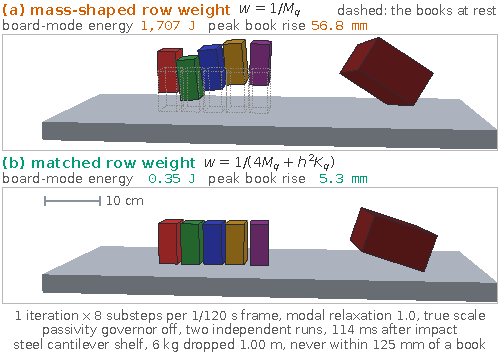
\includegraphics[width=0.95\columnwidth]{fig_onesweep_teaser.pdf}
\Description{Two stacked side views of the same shelf scene at the same instant,
drawn from one locked camera at true scale. In the upper panel, run with the
mass-shaped contact-row weight, the five standing books float clear of the shelf
surface, with dashed outlines marking where they had been resting, and the
dropped weight has bounced off the board. In the lower panel, run with the
reconstruction-matched contact-row weight, the same five books still stand on the
shelf and the dropped weight lies on it. Readouts above the panels give 1,707
joules of board-mode energy and 56.8 millimetres of peak book rise for the upper
panel against 0.35 joules and 5.3 millimetres for the lower one, and a footer
states the operating point both runs share.}
\caption{One shelf, one $6$~kg weight dropped $1.00$~m, one fixed budget
($1$ iteration $\times\ 8$ substeps per $1/120$~s frame); the arms differ only
in the modal contact row's weight. (a) The mass-shaped weight puts the row's
danger index above one and throws the five resting books off the
shelf, peak rise $56.8$~mm, at $1{,}707$~J of board-mode energy, not book
kinetic energy. (b) The
matched charge $\meff = m(\kappa^2 + (\oh)^2)$ at this host's
symplectic default $\kappa = 2$, priceable before the solve, holds them to
$5.3$~mm and $0.35$~J. Fixed-budget injection is a known
effect~\citep{wei2026earlyterm,giles2025avbd}; the weight is what differs. A
converged run on the same grid lifts a book $9.6$~mm, so (b) is not ground
truth.}
\label{fig:teaser}
\end{figure}

% =====================================================================
\section{Introduction}
% =====================================================================
A rigid-body position-based solver~\citep{mueller2020xpbd} already resolves
contacts and joints under a small, fixed local-iteration budget. To make a stiff
prop such as a shelf ring when struck, the light option is a
precomputed modal basis of a few global
amplitudes~\citep{james2002dyrt,peng2024softrobot} carried as extra unknowns in
the contact row that already couples the bodies: one host steps everything for
a handful of runtime numbers.

The difficulty is energetic (Fig.~\ref{fig:teaser}). A hard-constraint position
correction taken at a
fixed iteration budget ``can inject an arbitrary amount of
energy''~\citep{giles2025rtl}, and finite-iteration coupling can inject
spurious energy even when each coupled subsystem is passive on its
own~\citep{wei2026earlyterm}. Both are established observations, and this paper
claims neither. What a practitioner lacks is a way to predict, for a given row,
whether one sweep adds or removes energy, and what weight prevents it. A recent
solver comparison records the symptom without a framework: position
stabilization ``can lead to energy creation and jitter if not tuned
carefully''~\citep{catto2024solver2d}.

This paper is that framework for the shared unilateral contact-to-modal
row between a rigid body of mass $M$ and one restorative modal coordinate of
effective mass $m$ and frequency $\omega$, on the stiffness-blind
mass-normalized weight that position-based hosts default to. Every theorem
is confined to one Gauss-Seidel sweep from a cold start, with restitution
$e = 0$ and hard contact except where a compliance term appears.
Within that regime we contribute:

\begin{itemize}
\setlength{\itemsep}{0pt}\setlength{\parskip}{0pt}\setlength{\topsep}{2pt}
\item \textbf{C1.} A reconstruction-general one-sweep theorem
  (Thms.~\ref{thm:boundary} and~\ref{thm:exact}). For $\dot q^{+} =
  \kappa\,\Delta q/h$ the mass-only sweep injects exactly when $\kappa^2 +
  (\oh)^2 > 2 + m/M$; charging the restorative block at the matched operator
  $\kappa^2 M_c + h^2 K_c$, in both denominator and correction, makes one
  sweep passive for every $\kappa \neq 0$ and any number of coupled coordinates,
  and under hard contact it loses exactly a perfectly inelastic impact. Per mode this is
  $m(1 + (\oh)^2)$ at $\kappa = 1$, where one undamped matched sweep is exactly
  the converged implicit step, and $m(4 + (\oh)^2)$ at the shipped
  symplectic default
  $\kappa = 2$.
\item \textbf{C2.} The row-visible spectral form of that boundary at $\kappa = 1$,
  $h^2\,J M^{-1} K M^{-1} J^{\top} \succ J M^{-1} J^{\top}$
  (Thm.~\ref{thm:rowvisible}), reduced to a scalar danger index $\rho$ a host can
  evaluate per row before it solves; $\rho > 1$ is injection.
\item \textbf{C3.} A host-classification recipe and the relaxation boundary
  (Rmk.~\ref{rmk:recon}, Sec.~\ref{sec:guidance}): one cold sweep read back as
  $\Delta q/h$ or $2\Delta q/h$ fixes $\kappa$ and hence both the correct index
  and the matched weight, while under-relaxing the modal correction by $\theta$
  moves the boundary to $\theta^2(\kappa^2 + (\oh)^2) = 2 + m/M$.
\item \textbf{C4.} An ordering result (Prop.~\ref{prop:ordering}): a trailing
  restorative row divides the one-sweep modal deposit by $(1 + (\oh)^2)^2$ at
  every $\kappa$, which makes that order passive at $\kappa = 1$ but at
  $\kappa = 2$ only narrows injection to a low-stiffness band.
\end{itemize}

\noindent The diagnostic and the weight are row-local, not a global
safety mechanism: neither alone makes the solver passive.

% =====================================================================
\section{One-sweep model}
\label{sec:model}
% =====================================================================
\rih{Bodies and row.} A rigid body of mass $M$ presents a row-visible
mobility $\Rr$ (the scalar $1/M$ for a translational row; $\Rr = 1/M +
j_{a}^{\top} I^{-1} j_{a}$ for a full six-degree-of-freedom body). A restorative
modal coordinate $q$ has effective mass $m$, stiffness $k = m\omega^2$, and
damping $2\zeta\omega m$. The substep is $h$; we write $b = (\oh)^2 = h^2
k/m$ throughout. The unilateral hard contact row is $C = z - q \ge 0$, the rigid
gap minus the surface deflection, with multiplier $\lambda \ge 0$.

\rih{Local solve and reconstruction.} One Gauss-Seidel local solve of the
compliant row is
\begin{equation}
\Delta\lambda = \frac{-C - \tilde\alpha\lambda}{w + \tilde\alpha},
\qquad
\Delta x = M^{-1} J^{\top}\,\Delta\lambda,
\label{eq:localsolve}
\end{equation}
with $\tilde\alpha = \alpha/h^2$ the compliance and $w$ the row's weighted
mobility. Position-based hosts recover velocity from the position change;
backward Euler gives $\dot q^{+} = \Delta x / h$. Below, $\kappa$
rescales the \emph{restorative} read-back only; the rigid block recovers
$\Delta z/h$, as the shipped host does. One compliant row
solved once from rest is the exact backward-Euler step for its own spring, relaxing
a predicted $\tilde q$ to $\tilde q/(1 + b)$~\citep{macklin2016xpbd}.

\rih{Cold start and ledger.} A cold start has $q = \dot q = 0$, the contact
exactly touching, incoming gap rate $v < 0$, and predicted penetration
$\tilde C = h v$. Energies are the true Hamiltonian
\begin{equation}
E = \tfrac12 M v^2 + \tfrac12 m \dot q^2 + \tfrac12 k q^2
\label{eq:hamiltonian}
\end{equation}
at substep boundaries, and the sweep is \emph{injecting} when $E^{+} > E^{-}$.
Since a passive unilateral contact cannot raise $E$ and the converged step is
dissipative~\citep{anitescu1997lcp}, any one-sweep increase is a truncation
artifact by definition, not a property of the contact model.

\rih{Scope (stated once, binds every theorem).} One Gauss-Seidel
sweep; cold start; restitution $e = 0$; hard contact except where $\tilde\alpha$
appears; one coupling row; normal-only, no friction.

% =====================================================================
\section{Results}
\label{sec:results}
% =====================================================================

\begin{theorem}[Scalar sign boundary, C1]
\label{thm:boundary}
Under the scope of Section~\ref{sec:model}, mass-only weight $\wm = M^{-1} +
m^{-1}$ and backward-Euler reconstruction, one projection of the cold-start row
satisfies
\begin{equation}
E^{+} = \tfrac12 v^2 \Big(\tfrac{M}{M+m}\Big)^{\!2}\big[\,M + m + m(\oh)^2\,\big],
\qquad E^{-} = \tfrac12 M v^2,
\label{eq:eplus}
\end{equation}
and hence $E^{+} > E^{-}$ if and only if $(\oh)^2 > 1 + m/M$.
\end{theorem}

\begin{proof}
The cold prediction is $\tilde C = h v$, so \eqref{eq:localsolve} with
$\tilde\alpha = 0$ gives $\Delta\lambda = -h v / \wm$ and, the relative normal
rate being zeroed, the inelastic-pair reconstruction
$v^{+} = \dot q^{+} = v M/(M+m)$, $q^{+} = h\dot q^{+}$. Substituting into
\eqref{eq:hamiltonian} and clearing $Mm > 0$ reduces $E^{+} > E^{-}$ to
$(\oh)^2 > 1 + m/M$.
\end{proof}

At equality the projection is exactly energy-neutral; for $m \ll M$ the boundary
is $\oh = 1$. The offset
$1 + m/M$ distinguishes it from the penalty-contact Courant limit at
$(\oh)^2 \sim \mathcal{O}(1)$.

% Single column: the graphic's MediaBox is 241.147 bp, i.e. one \columnwidth, so
% it prints at 0.996x and its smallest glyph, a mathtext subscript, reaches the
% page at 6.07 pt. It no longer carries the caption-duplicating title and footer
% bands, so the previous trim/clip is gone. Built by make_figs_singlecol.py from
% the same out/t2_phasemap.csv as before; no plotted quantity changed.
\begin{figure}[t]
\centering
% Trim: the graphic's bottom legend band ("analytic boundary (wh)^2 = 1 + m/M")
% is word-for-word the caption's own identification of the solid curve. Measured
% on a 200 dpi render: the band occupies the bottom 13 pt, the omega-h axis
% labels end 6 pt above it, so nothing else is touched.

\includegraphics[trim=0 13 0 0,clip,width=\columnwidth]{fig_onesweep_phase_map.pdf}
\Description{Two heatmaps of signed energy change over the omega-h and mass-ratio
plane. The mass-only weight panel shows a red injection region lying exactly
above the plotted analytic boundary curve; the implicit weight panel is blue
everywhere.}
\caption{Phase map over $(\oh,\ m/M)$. Left, the mass-only
weight injects (red) exactly where the solid analytic curve
$(\oh)^2 = 1 + m/M$ predicts; right, the implicit weight is passive (blue). Hard
contact, one sweep, cold start, $e = 0$, $\kappa = 1$.}
\label{fig:phasemap}
\end{figure}

\begin{theorem}[Row-visible condition, C2]
\label{thm:rowvisible}
Let the row span a rigid block (mobility $\Rr$) and modal coordinates with
$a_i = U_i^2/m_i$ and $b_i = (\omega_i h)^2$. Under the scope of
Section~\ref{sec:model} with mass-only weights and $\kappa = 1$,
\begin{equation}
\Delta E = \frac{v^2}{\wm^2}\Big(\tfrac12 \wE - \wm\Big),
\quad \wm = \Rr + \textstyle\sum_i a_i,
\quad \wE = \wm + \textstyle\sum_i a_i b_i,
\label{eq:r4}
\end{equation}
so the sweep injects if and only if
\begin{equation}
\textstyle\sum_i a_i b_i > \Rr + \sum_i a_i
\;\Longleftrightarrow\;
h^2\, J M^{-1} K M^{-1} J^{\top} \succ J M^{-1} J^{\top}.
\label{eq:spectral}
\end{equation}
Writing $L = \sum_i a_i b_i = h^2 J M^{-1} K M^{-1} J^{\top}$, the row danger
index $\rho = L/\wm$ satisfies $y := 2\,\Delta E\,\wm/v^2 = \rho - 1$ exactly, so
injection is the single condition $\rho > 1$. A compliance $\tilde\alpha$ shifts
it to $\rho = L/(\wm + 2\tilde\alpha)$.
\end{theorem}

The right-hand operator of \eqref{eq:spectral} is the Delassus, or inverse
operational-space inertia, that contact solvers already form as an interface
effective mass~\citep{andrews2019schur,peiret2018interface}; the left-hand one
reflects the material stiffness twice through the same row. Neither is new; the
contribution is reading their ordering as the sign of one-sweep energy transfer.
Because $\rho$ lives in physical coordinates, \eqref{eq:spectral} is not an
artifact of any modal basis, as Section~\ref{sec:validation} confirms.
Here $J$ is one row, so $\succ$ is the scalar $L > \wm$;
Thm.~\ref{thm:exact} gives the operator form for many coordinates sharing the
row, and several \emph{simultaneously active} rows are outside our scope,
measured in Section~\ref{sec:guidance}.

\begin{theorem}[Reconstruction-matched effective mass, C1]
\label{thm:exact}
Under the scope of Section~\ref{sec:model} but with any number of coupled
restorative coordinates, let the block have mass $M_c \succ 0$ and stiffness
$K_c \succeq 0$, let the row price it at a charge operator $W$ used in both the
denominator of \eqref{eq:localsolve} and the position correction, and let the
restorative velocity be reconstructed as $\dot q^{+} = \kappa\,\Delta q/h$ and
the rigid one as $\Delta z/h$. Write
$G = \kappa^2 M_c + h^2 K_c$ and $u = W J_c$. Then one sweep changes the energy by
\begin{equation}
\Delta E = \frac{v^2}{2 D^2}\big[\,u^{\top} G\, u - \Rr
  - 2 J_c^{\top} u - 2\tilde\alpha\,\big],
\qquad D = \Rr + J_c^{\top} u + \tilde\alpha,
\label{eq:c3general}
\end{equation}
so it injects if and only if $u^{\top} G u > \Rr + 2 J_c^{\top} u +
2\tilde\alpha$. The reconstruction-matched charge $W = G^{-1}$ makes
$u^{\top} G u = J_c^{\top} G^{-1} J_c$ telescope, giving
\begin{equation}
\Delta E = -\frac{v^2}{2 D^2}\,\big(\Rr + J_c^{\top} G^{-1} J_c
  + 2\tilde\alpha\big) \;<\; 0
\label{eq:c3}
\end{equation}
unconditionally, for every $\kappa \neq 0$, every $M_c \succ 0$, every
$K_c \succeq 0$ and every $\tilde\alpha \ge 0$. At $\tilde\alpha = 0$,
\eqref{eq:c3} is $-\tfrac12 [M m_{\mathrm{row}}/(M + m_{\mathrm{row}})] v^2$
with $m_{\mathrm{row}} = 1/(J_c^{\top} G^{-1} J_c)$, the energy lost in the
perfectly inelastic impact of the pair $(M, m_{\mathrm{row}})$.
\end{theorem}

For one coordinate and $\tilde\alpha = 0$, $u^{\top} G u > \Rr +
2 J_c^{\top} u$ reads
$M m(\kappa^2 + b) > 2 M \mu_c + \mu_c^2$ for a scalar charge $\mu_c$, the
matched charge is $\meff = m(\kappa^2 + b)$, and \eqref{eq:c3} is
$-\tfrac12[M\meff/(M+\meff)]v^2$: $m(1 + b)$ under backward Euler
($\kappa = 1$), $m(4 + b)$ under the symplectic default
($\kappa = 2$). Thms.~\ref{thm:boundary} and~\ref{thm:rowvisible} are its
$W = M_c^{-1}$, $\kappa = 1$ specializations.

One scalar weight per mode realizes $G^{-1}$ exactly when $G$ is diagonal, that
is whenever $K_c$ is, as in a modal basis. The hypothesis is not cosmetic:
charging only the diagonal of $G$ when
$K_c$ has off-diagonal entries breaks \eqref{eq:c3}, injecting on $19$ of $2000$
randomized coupled-stiffness rows where full $G^{-1}$ stays passive on all.
Diagonal, $G^{-1}$ is $r$
reciprocals per substep and leaves the row solve at $0.99$ to $1.02$ times the
mass-only default; coupled, it needs one Cholesky of $G$, refactored per substep in our reference, and $2r^{2}$ flops per row
against $2r$, $6.8$ to $14.5$ times the diagonal accumulation for $r = 4$ to
$64$, ratios on a reference implementation, not production timings.

\begin{corollary}[Passive family, C1]
\label{cor:family}
Under the hypotheses of Theorem~\ref{thm:exact} with $W$ symmetric, one sweep is
passive for every row $J_c$ if and only if $0 \preceq W \preceq 2G^{-1}$ in the
Loewner order.
On the ray $W = cG^{-1}$, with $a = J_c^{\top} G^{-1} J_c \ge 0$,
\eqref{eq:c3general} collapses to
\begin{equation}
\Delta E = \frac{v^2}{2D^2}\big[\,c(c-2)\,a - \Rr - 2\tilde\alpha\,\big],
\quad D = \Rr + c\,a + \tilde\alpha,
\label{eq:family}
\end{equation}
so every $c \in [0,2]$ is passive unconditionally, and outside that interval the
row injects once $a > (\Rr + 2\tilde\alpha)/[c(c-2)]$.
\end{corollary}

The matched charge is the interior point $c = 1$; the far
endpoint $c = 2$ is the scalar charge $G/2$, which in one coordinate at
$\kappa = 2$ is $m(2 + b/2)$: the converged amplitude that $c = 1$ misses
(Section~\ref{sec:validation}) is recovered exactly and passively there. Of $2500$ randomized symmetric charges
met with adversarial rows, all $1222$ inside the interval are
passive and all $1278$ outside inject (T14a).

\eqref{eq:c3general}
accounts for the position \emph{projection} only and $E$ is the undamped
Hamiltonian: the damper acts in the predictor, so its non-positive contribution
is neither charged nor relied on; the bound is the conservative half of the
step. $E$ counts the bodies only: a compliant row also stores
$\tilde\alpha v^2/(2D^2)$ in its own spring, so counting that term tightens
each $2\tilde\alpha$ threshold to $\tilde\alpha$, a band on which the displayed
ledger is permissive; no sign reported here changes, and the matched charge
stays passive either way, at $-(v^2/2D^2)(\Rr + a + \tilde\alpha)$.
The two masses damping produces must not be conflated: the matched
charge $\meff = m(\kappa^2 + b)$ is the \emph{stored-energy} mass,
damping-independent, and keeps \eqref{eq:c3} exact at any $\zeta$ because a cold
predictor is inert and the damper stores nothing, whereas the \emph{per-impulse}
mass, $m(1 + 2\zeta\oh + b)$ at $\kappa = 1$ and $m(1 + \zeta\oh + b/4)$ at
$\kappa = 2$, is strictly inside passivity at
$\kappa = 1$ and unmatched at $\kappa = 2$. The loss form of \eqref{eq:c3} is the
classical reduced-mass shock loss~\citep{moreau1985shocks},
$(M + hD + h^2 K)^{-1}$ is the linearized implicit-step mobility whose stiffness
term solvers routinely drop~\citep{tournier2015stable,andrewserleben2017geometric}, and
$1 + (\oh)^2$ is the backward-Euler propagator; we claim none of these. Ours is
the effective mass a truncated row charges under general reconstruction, and
the identity that one matched sweep is exactly that inelastic
impact. The converged step being already
passive~\citep{anitescu1997lcp}, the statement lives only in the truncated regime.\looseness=-1

Under the shipped convention the relaxation $\theta$ multiplies only the
modal position correction, leaving the multiplier and rigid update at full
strength. The modal deposit then scales as $\theta^2$ with the rigid loss
unchanged, so the mass-arm boundary becomes $\theta^2(\kappa^2 + b) > 2 + m/M$:
under-relaxation raises the threshold and can move a marginally injecting sweep
to passive, never the reverse. Relaxing the whole correction, rigid and modal,
gives $L > (2/\theta - 1)\wm$.

\begin{proposition}[Ordering divisor, C4]
\label{prop:ordering}
Take two rows on $(z, q)$: the contact $C_c = z - q$ (hard, unilateral) and a
compliant spring $C_s = q$ with $\tilde\alpha_s = 1/(k h^2)$. At $n = 1$ from a
cold start, order $A = [\text{contact}, \text{spring}]$ and order $B =
[\text{spring}, \text{contact}]$ deposit modal energies $D_A, D_B$ with
$D_B/D_A = (1 + b)^2$ at every $\kappa$, and order $A$ injects exactly when
$(\kappa^2 + b)/(1+b)^2 > 2 + m/M$.
\end{proposition}

Order $B$ leaves the spring a no-op from rest and reproduces
Thm.~\ref{thm:boundary}; order $A$ deposits a fresh $q_c$ that the trailing
spring relaxes to $q_c/(1+b)$, cutting the deposit by $(1+b)^2$, so its
injection condition is Thm.~\ref{thm:boundary}'s divided by that factor. At
$\kappa = 1$ the left side is $1/(1+b) \le 1 < 2 + m/M$, so that
order is one-sweep passive at every stiffness and mass ratio. The add-on does
not survive $\kappa = 2$: with $s = 2 + m/M$ the condition
$s b^2 + (2s - 1) b + s - \kappa^2 < 0$ has a positive root $b^{*}$
exactly when $m < (\kappa^2 - 2)M$; order $A$ then
injects on $b < b^{*}$ by at most $(\kappa^2 - 2)^2/[4(\kappa^2 - 1)]$ of the
incoming kinetic energy. At $\kappa = 2$ that is $m < 2M$, with
$b^{*} = (\sqrt{37} - 5)/6 = 0.180$ at $m = M$ and a third of $E^{-}$ at worst.
That Gauss-Seidel order affects energy is
known~\citep{arnold2010stability,cetinaslan2019energyaware}, and the
compliant-row-equals-backward-Euler premise is
Macklin~et~al.'s~\citep{macklin2016xpbd}; the closed-form $(1 + (\oh)^2)^2$
divisor and the reconstruction-scoped condition are ours.\looseness=-1

\begin{remark}[Reconstruction dependence]
\label{rmk:recon}
Thms.~\ref{thm:boundary} and~\ref{thm:rowvisible} are stated at
$\dot q^{+} = \Delta q/h$. The shipped host default is a symplectic
implicit-midpoint stepper reconstructing $\dot q^{+} = 2\Delta q/h - \dot q^{n}$,
that is $2\Delta q/h$ at a cold start (measured exact on the shipped arrays),
depositing four times the backward-Euler modal kinetic
energy. Which block carries $\kappa$ decides the boundary: scaling the rigid
read-back by $\kappa_r$ too weights the $\Rr$ term of \eqref{eq:c3general}
by $\kappa_r(2 - \kappa_r)$ and the $J_c^{\top}u$ and $\tilde\alpha$ terms by
$\kappa_r$, so mass-only injection is
$\kappa^2 + b > 2\kappa_r + \kappa_r(2 - \kappa_r)\,m/M$:
$b > 1 + m/M$ at $(\kappa_r, \kappa) = (1,1)$; $b > m/M - 2$ at $(1,2)$,
injecting at \emph{every} stiffness once $m < 2M$; and $b > 0$ at $(2,2)$. The
matched charge is passive for every $\kappa \neq 0$ at Thm.~\ref{thm:exact}'s
$\kappa_r = 1$, and under $\kappa_r = \kappa$ at every mass ratio if and
only if $\kappa \in [1/2, 2]$. A weight
matched to the wrong reconstruction is not passive either: the backward-Euler
weight $m(1+b)$ on a $\kappa = 2$ host injects whenever $M(2 - b) > m(1+b)^2$,
the low-stiffness injection measured in Section~\ref{sec:validation}.\looseness=-1
\end{remark}

\begin{figure*}[t]
\centering
% Crop: as above, the graphic's suptitle and its five-line footer restate this
% caption. Clearance re-measured on a 150 dpi render of the graphic: panel
% titles start 43.2 pt from the top (trim 40) and the x-axis labels end 379 pt
% down (trim bottom 74 of 457.9), so every panel title, axis, legend and inset
% survives and the previously half-clipped first footer line is now gone.

\includegraphics[trim=0 74 0 40,clip,width=0.88\textwidth]{fig_onesweep_rowindex.pdf}
\Description{Three scatter panels of measured one-substep energy change against a
danger index for a shipped contact row. In the backward-Euler control panel the
sign flips at index one. In the symplectic-default panel the sign flips at the
shifted midpoint index and the backward-Euler-shaped implicit weight injects. In
the reconstruction-matched panel the matched weight stays below zero at every
danger index while the unmatched weight injects.}
\caption{Shipped position-based contact row. Left, backward-Euler control.
Middle, host default, where the reconstruction shifts the governing index to
$\rho_{\mathrm{mid}}$ and the backward-Euler-shaped weight injects. Right, the
matched weight $4 M_q + h^2 K_q$; inset, injection decays as the
budget grows. Hard contact, one sweep, cold start, $e = 0$.}
\label{fig:rowindex}
\end{figure*}

% =====================================================================
\section{Validation}
\label{sec:validation}
% =====================================================================
\rih{Relation to the companion study.} A companion submission under
review~\citep{companion2026diagnosis} is a system-level diagnostic: it measures
injection and runs a weight-swap control on a production host, with no closed
forms. This paper is the per-sweep closed-form theory. Shared evidence is
confined to the host and to two arms of the $24$-cell weight swap below,
mass-only and $(M_q + hD_q + h^2K_q)^{-1}$; everything else is new, including
the $27$-cell shipped-row test and the matched arm.

Every closed form above was checked numerically by the suite of
Table~\ref{tab:validation}; the toy and nonmodal models are structurally
independent code paths from the analytic forms, so a shared implementation error
would not agree across them, and the operator identity is verified in exact
rational arithmetic. The attached anonymous supplement ships every check in that
table with its per-cell CSV: runnable code for the analytic arms, drivers and
host excerpts for the shipped-host ones. The one loose tolerance is T4, the
shipped row: its mass arm reproduces the backward-Euler identity to the
$10^{-3}$ magnitude band, while the implicit arm is validated at sign and
passivity level, its magnitude deviating up to $4.5\times10^{-2}$ from two slack
sources named in advance, quaternion second-order terms and the velocity pass.

\begin{table}[t]
\centering
\small
% The caption is a definitions block for six column headings plus three
% qualifiers, so it is long by necessity; setting it one step down keeps every
% definition and every qualifier and returns about 4 typeset lines. Only this
% one caption is affected; figure captions stay at the class default.
\captionsetup{font=small}
\caption{Validation suite. \emph{Model}: \emph{analytic} a
closed-form row, \emph{nonmodal} a mass-spring chain, \emph{shipped} a
production solver. \emph{Cells} counts independent parameter
draws, each possibly run under several weights or reconstructions.
\emph{Crit.} is the per-cell test: a relative residual bound, \emph{sign} for
predicted vs.\ measured energy sign, \emph{exact} for rational
equality, or \emph{ratio} for T6, where a cell \emph{overruns} when its peak
modal energy exceeds the impactor's peak rigid kinetic energy. Under
\emph{Result}, \emph{checks} counts named assertions over a block's cells;
other entries count cells, out of \emph{Cells} unless a denominator is given;
T4, T6, T13, T14b give one per arm. Signs are undefined where the predicted
change vanishes; cells within $10^{-9}$ of it are non-live: none
in T2, T5, T7, T13, $12$ of T3's $300$, all with
$|\Delta E| \le 2.3\times10^{-16}E^{-}$. T4's pair uses a backward-Euler
control; the host default is Fig.~\ref{fig:rowindex}. Only T10's $300$ and
T14a's $720$ rational cells are exact; their float cells are
conditioning-limited at $10^{-9}$.}
\label{tab:validation}
\setlength{\tabcolsep}{3pt}
\footnotesize
\begin{tabular}{@{}llllll@{}}
\toprule
 & What & Model & Cells & Crit. & Result \\
\midrule
T1 & Identity battery & analytic & $2626$ & $10^{-12}$ & $29/29$ checks \\
T2 & Phase map & analytic & $58{,}081$ & $10^{-12}$, sign & $0$ misclass. \\
T3 & Nonmodal collapse & nonmodal & $300$ & $10^{-12}$, sign & $288/288$ live \\
T4 & Shipped row & shipped & $2{\times}27$ & sign & $27/27$, $27/27$ \\
T5 & Ordering, converged & analytic & $208$ & $10^{-12}$ & $184/184$ checks \\
T6 & Weight swap & shipped & $3{\times}24$ & ratio & $8/0/0$ overrun \\
T7 & Recon.\ mass law & analytic & $7000$ & $10^{-12}$, sign & $0$ mismatch \\
T8a & Relax.\ boundary & analytic & $1200$ & $10^{-12}$, sign & $0$ mismatch \\
T8b & Relax.\ direction & analytic & $1600$ & sign & $0$ unsafe flips \\
T9 & Matched arm & shipped & $27$ & sign & $27/27$ passive \\
T10 & Operator form & analytic & $9900$, $300$ & $10^{-9}$; exact & $17/17$ checks \\
T11 & Converged reference & analytic & $15{,}000$ & $10^{-12}$ & $8/8$ checks \\
T12 & Hypothesis pinning & analytic & $53{,}000$ & $10^{-12}$, sign & $28/28$ checks \\
T13 & Ordering vs.\ $\kappa$ & analytic & $2{\times}10^{4}$ & $10^{-12}$, exact & $0$, $3840$ inject \\
T14a & Charge family & analytic & $2100$, $720$ & $10^{-9}$; exact & $0$ inject in $[0,2]$ \\
T14b & Equal cost & shipped & $12{\times}27$ & sign & $22$ vs.\ $0$ inject \\
T14c & Warm, two-row & analytic & $43{,}783$ & sign & $2795$ unsafe \\
\bottomrule
\end{tabular}
\end{table}

\rih{Phase map (Fig.~\ref{fig:phasemap}).} A $241 \times 241$ grid in
$(\oh,\ m/M)$, measured by the one-sweep projection rather than the closed form,
misclassifies no cell against $(\oh)^2 = 1 + m/M$.

\rih{Nonmodal collapse (Fig.~\ref{fig:nonmodal}).} We repeat the
measurement in plain point-mass and spring coordinates, no modal basis anywhere,
over four variants including a wide plank row that exercises the off-diagonal of
$K$ through $J M^{-1} K M^{-1} J^{\top}$. All $288$ live cells agree in sign with
$\rho > 1$, and every variant collapses onto $y = \rho - 1$ to
$4.3 \times 10^{-14}$.

\rih{Ordering.} The two-row toy confirms Prop.~\ref{prop:ordering}: at $n = 1$ the
ratio $D_B/D_A = (1+b)^2$ is exact, $10201$ at $b = 100$.
Carrying $\kappa$ through the toy on $10{,}000$ cells per reconstruction
(T13) leaves that order passive on all at $\kappa = 1$ and
injecting on $3840$ at $\kappa = 2$, which at the shipped $h = 1/960$~s substep
is every mode below $65$~Hz at $m = M$. Both orders reach the same converged backward-Euler
point, dissipative when read back at $\kappa = 1$, monotonically from opposite
sides.

\rih{Accuracy against a converged reference.} Passivity is a weak
certificate: over-dissipating is passive too. We compare each arm against the
exactly solved converged implicit contact step, on contact impulse, post-step
rigid velocity, modal amplitude and modal velocity (T11).
First, the constraint residual cannot discriminate: one sweep of a single
row drives $C^{+}$ to zero for \emph{every} weight, since
$\Delta C = w\,\Delta\lambda = -C$, measured at $2.1\times10^{-16}$ of $|hv|$ across
$32{,}000$ arm-cells. Second, at $\kappa = 1$ and $\zeta = 0$ the matched weight
reproduces the converged backward-Euler step \emph{exactly}, to
$5.5\times10^{-16}$ relative on all four quantities. With
damping the amplitude gap is exactly $2\zeta\oh/(1 + M/m + b)$, first order in
$\zeta\oh$ over four decades and $0.979\,\zeta\oh$ at the measured $m = M$,
$b = 0.043$. Third, still at $\kappa = 1$, the mass-only arm's
defect has an accuracy face: it over-deposits the modal amplitude by exactly
$(M + m(1+b))/(M+m) = 1 + b\,m/(M+m)$, which at $m = M$ is
$51$ at $b = 10^{2}$ and $5001$ at $b = 10^{4}$, the same
$(\oh)^2$ that drives the sign boundary. Fourth, the
reference at $\kappa = 2$ is the host's own converged step, the mode on implicit
midpoint with the row at position level, so $v^{+} = \dot q^{+}/2$ and
the row reproduces it at $\mu_{\ast} = m(2 + b/2)$. The matched
charge $m(4+b)$ is exactly $2\mu_{\ast}$, so it over-dissipates: the amplitude
ratio is $(M + \mu_{\ast})/(M + 2\mu_{\ast})$, falling to $1/2$ only as
$\mu_{\ast}/M \to \infty$, and it is never less dissipative than the reference
on any of $3000$ cells. Passive and conservative, not accurate.\looseness=-1

\rih{Shipped contact row (Fig.~\ref{fig:rowindex}).} We drive one
cold-start row of a production position-based support solver, the host of the
companion study~\citep{companion2026diagnosis}, on its three scenes, with the
passivity governor off, relaxation at $1$ and no other contacts, nine stiffness
points per scene across many decades of $\rho$ ($27$ cells), under both the host
default reconstruction and a backward-Euler control.
Under the control the mass-arm sign matches $\rho > 1$ on all $27$ cells and the
backward-Euler remedy is passive on all $27$. Under the
host default (Rmk.~\ref{rmk:recon}) the governing index is the
$\kappa = 2$ instance of Thm.~\ref{thm:exact}, which for mass-only weights reads
$\rho_{\mathrm{mid}} = (L + 2\sum_i a_i)/(\Rr + 2\tilde\alpha)$: $\sum_i a_i$
moves from the denominator to the numerator, so this is not a rescaling of
$\rho$. It tracks the measured mass-arm sign on all $27$ cells, whereas $\rho$
tracks only $22$, and the five misses are false \emph{negatives}, the unsafe
direction for a pre-solve check: a safe row that measurably injects, at the
softest modes of the two strongly coupled scenes. The backward-Euler-shaped
remedy, no longer matched to the reconstruction, stays passive only where the
coupling is weak (dinner $9/9$; shelf $2/9$, ledge $4/9$), while the matched
weight $m(4 + (\oh)^2) = 4 M_q + h^2 K_q$ is passive on every cell, its danger
index below one throughout, at the same operating points where the unmatched
weight injects.

\rih{System-level corroboration.} The $24$-cell weight-swap grid of the
companion study~\citep{companion2026diagnosis} runs a production host across
three scenes, two relaxations $\theta \in \{0.7, 1.0\}$, and four
iteration-substep budgets $(4,1)$, $(8,2)$, $(16,4)$, $(32,8)$, read as
iterations $\times$ substeps per $1/120$~s frame, so $h$ runs from $1/120$ to
$1/960$~s, with the symplectic stepper and the passivity governor off (hard
contact; cold impacts onto warm, simultaneous support rows, beyond the
one-sweep scope). We re-run
it with a third arm. Under the stiffness-blind mass-only weight $8$ of $24$ cells
overrun, their peak modal energy exceeding the measured rigid-side supply by up
to $1.2 \times 10^{5}$ at the lowest budget. The ratio is a gross-overrun test;
the total-energy sign gives $10$, $1$ and $0$ of $24$ across the three arms. Under the
weight $(M_q + hD_q + h^2K_q)^{-1}$ none do ($0$ of $24$), which is the
companion's published arm; but that weight is shaped for $\kappa = 1$ while this
host reconstructs at $\kappa = 2$, so by Thm.~\ref{thm:exact} it is \emph{not}
the matched weight here and its success is evidence about stiffening the row, not
about the one-sweep identity. The arm that does test the theorem charges
$4M_q + h^2K_q$, also overrun-free ($0$ of $24$) and lying strictly below the
$\kappa = 1$ arm on every cell, consistent with the over-dissipation predicted
for $\kappa = 2$. The eight overrunning cells are exactly the two strongly
coupled scenes at the two lowest budgets and both relaxations, matching
Theorem~\ref{thm:boundary}'s coupling-strength dependence. Our mass-only arm
reproduces the companion's published ratios exactly on all
$24$ cells, so the two grids are the same experiment.\looseness=-1

\begin{figure}[t]
\centering
% Trim: 8 pt of empty bottom margin below the x-axis label and 6 pt to the right
% of the axes box, measured on a 200 dpi render; no glyph is touched.
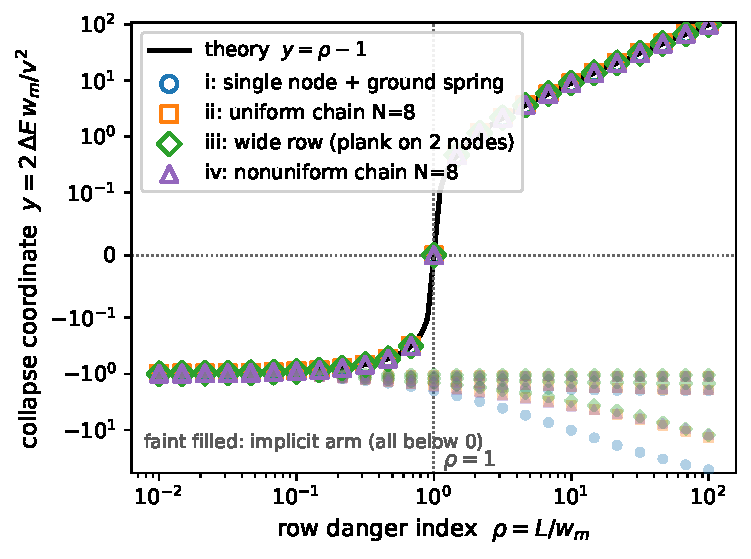
\includegraphics[trim=0 8 6 0,clip,width=0.76\columnwidth]{fig_onesweep_nonmodal.pdf}
\Description{Scatter plot of the collapse coordinate against the row danger index
on log axes. Points from four mass-spring variants all fall on the straight
theory line that crosses zero at danger index one; a faint second series sits
entirely below zero.}
\caption{Nonmodal collapse: four mass-spring variants on
$y = \rho - 1$ of Thm.~\ref{thm:rowvisible}; the faint implicit arm is
negative.}
\label{fig:nonmodal}
\end{figure}

\rih{Is the weight worth its budget?} At fixed
stiffness injection decays to passivity by four to eight iterations
(Fig.~\ref{fig:rowindex}, inset), but across all $27$ cells more
slowly: iterating the mass-only weight leaves $17$,
$9$, $6$ and $2$ cells injecting at $2$, $4$, $8$ and $16$. The last still
overshoots one cell by $28$ times its incoming kinetic energy at $5.3$ times
the measured substep cost, whereas the matched weight is passive on all $27$ at
$0.996$ of the mass-only cost. What iterating converges to is
the reference, not the guarantee: passive on all $27$ at $64$ iterations and
$20$ times the cost. The guarantee is paid for in amplitude instead, a median
$0.57$ of the converged against $0.85$ at $16$ iterations (T14b).

% =====================================================================
\section{Related work}
\label{sec:related}
% =====================================================================
\rih{Co-simulation stability and energy residuals.} The two-mass
oscillator is the canonical co-simulation stability model, but its boundaries are
asymptotic spectral-radius conditions on a macro-step amplification
matrix~\citep{kubler2000coupling,gomes2018cosim}, not
per-sweep energy signs, and Arnold's sequential-coupling stability
analysis~\citep{arnold2010stability} is a contractivity condition, not a
closed-form deposit factor. Energy-sign framings of coupling error exist as
runtime residuals for adaptive step control~\citep{sadjina2016power} and as
energy-leak monitoring~\citep{gonzalez2019energyleak}, again not
parametric thresholds; the interface effective-mass operator behind our
$\rho$ serves elsewhere as a stabilizing predictor~\citep{peiret2018interface}.
C1, C2 and C4 are the closed-form, per-sweep, unilateral-row content those
programs lack.

\rih{Graphics constraint solvers.} Position-based dynamics establishes the
compliant-row premise and the stiffness-blind default
weight~\citep{macklin2016xpbd}, and single-iteration substepping targets energy
loss, not gain~\citep{macklin2019small}. Reduced deformable coordinates have
been carried inside a position-based host as extra degrees of
freedom~\citep{peng2024softrobot}, so stepping modal amplitudes in the solver is
established practice; we claim neither the coupling nor the embedding. Augmented
vertex block descent concedes hard-constraint injection and mitigates it
empirically~\citep{giles2025avbd}, building on~\citet{chen2024vbd}, and
energy-aware Gauss-Seidel studies
within-solve energy~\citep{cetinaslan2019energyaware}, but none gives a closed-form
sign boundary or a one-sweep passivity identity; practitioner accounts
report the symptom and prescribe tuning~\citep{catto2005iterative,catto2024solver2d}.

\rih{Contact mechanics endpoints and reduced coordinates.} The reduced-mass
shock loss~\citep{moreau1985shocks} and the dissipativity of the converged
solve~\citep{anitescu1997lcp} bound the endpoints our one-sweep
statement sits between. Reduced-coordinate contact
against internal modes has been posed as a momentum-conserving remapping without
an energy bound~\citep{sheth2015}, and energy targets set at the whole-system
rather than per-row level~\citep{you2026energy}. The closest guarantee is
finite-iteration
coupling that builds in discrete passivity for any inner budget on bilateral
interfaces~\citep{wei2026earlyterm}; ours is orthogonal, a sign diagnostic and
weight for a unilateral row rather than automatic passivity.

% =====================================================================
\section{Practitioner guidance and limitations}
\label{sec:guidance}
% =====================================================================
\rih{When to couple into the row.} Coupling the mode into the row is one
design point. A stiff prop can instead ring from an open-loop modal bank
driven by the solver's own impulse, the standard route in
contact-sound synthesis, which sidesteps injection: the
mode never enters the row. In-solve coupling is needed when a second object rests
persistently on the deforming region while it rings, cargo on a shelf or a plank
on a ledge: the deflection is then at or above the contact tolerance, and a bank
that never updates it prices support impulses against a stale surface. Open-loop
excitation stays the safer default for audio-rate ringing and unloaded props.

\rih{Recipe.} \emph{(i)~Classify.} Drive one cold row and read back the
restorative velocity: $\Delta q/h$ is $\kappa = 1$, $2\Delta q/h$ is
$\kappa = 2$; Thm.~\ref{thm:exact} reads the rigid block at $\Delta z/h$, and
if the host rescales that block too, use Rmk.~\ref{rmk:recon}'s boundary.
\emph{(ii)~Test before solving:} with $\Rr$, $a_i$, $b_i$ and $L$ of
Thm.~\ref{thm:rowvisible}, mass-only weights inject exactly when
$\rho_{\kappa} = [L + (\kappa^2 - 2)\sum_i a_i]/(\Rr + 2\tilde\alpha) > 1$;
$\rho_{\mathrm{mid}}$ is its $\kappa = 2$ instance, and evaluating it costs
$6\%$ of the row solve it precedes. \emph{(iii)~Charge} the restorative block at
$W = (\kappa^2 M_c + h^2 K_c)^{-1}$ in the denominator of \eqref{eq:localsolve}
\emph{and} in the position correction; the denominator alone is not the proved
method. \emph{(iv)~Factor once:} a diagonal $K_c$, as in a modal basis, makes
$W$ $r$ reciprocals with no matrix assembled; when $K_c$ couples, one Cholesky
of $G$ is shared across rows and, the basis and $h$ being fixed, hoists to load
time. \emph{(v)~Choose the family point:} the matched charge
is $c = 1$ of Cor.~\ref{cor:family}, per mode $m(\kappa^2 + (\oh)^2)$. At a low
budget it rings more weakly
than the mass-only arm's over-deposit, so a stronger ring means iterating the
row, decoupling to open-loop excitation, or moving toward $c = 2$, which returns the converged amplitude exactly
where $c = 1$ returns $0.50$ to $0.60$ of it, at the cost of margin: headroom to
the injection threshold falls under $1\%$ on a fifth of the cells measured
(median $36\%$) against at least $100\%$ at $c = 1$ (median $171\%$). A
mis-estimated $G$ is the same family at $c\,G/\hat{G}$, so $c = 1$ absorbs any
overestimate of $G$ and a twofold underestimate, while $c = 2$ loses the
guarantee under any underestimate; keep $c = 1$ unless the ring amplitude
is the deliverable (T14a).
Not matching leaves weak coupling ($2\sum_i a_i \le \Rr$), iterating to
convergence, or under-relaxing, a partial mitigation rather than a substitute.\looseness=-1

\rih{Limitations.} Section~\ref{sec:model}'s scope binds every theorem, the
reconstruction included: ordering the restorative row after the contact row is a
passivity fix at $\kappa = 1$ only, and on the symplectic default it leaves the
low-stiffness band of Prop.~\ref{prop:ordering}. Warm states and simultaneously
active rows are measured, not proved (T14c): the mass-only weight itself injects
on $19{,}730$ of $43{,}783$ warm and two-row cells, $2795$ of them called safe by
its index, and order alone flips $734$ signs; the matched charge, clean under the
shipped $\kappa = 2$ midpoint pairing and secularly bounded over $20{,}000$
substeps of resting contact, still injects on $4099$ of $43{,}898$, a measured
reduction and not a guarantee (the denominators differ because row activity after
the sweep depends on the weight; both arms scan the same draws). The interior
$1 < n < \infty$,
restitution and friction are open.\looseness=-1

\bibliographystyle{ACM-Reference-Format}
\bibliography{references,onesweep_refs}

\end{document}
